% **************************************************
% Document Class Definition
% **************************************************
\documentclass[%
    paper=A4,               % paper size --> A4 is default in Germany
    twoside=true,           % onesite or twoside printing
    openright,              % doublepage cleaning ends up right side
    parskip=full,           % spacing value / method for paragraphs
    chapterprefix=true,     % prefix for chapter marks
    11pt,                   % font size
    headings=normal,        % size of headings
    bibliography=totoc,     % include bib in toc
    listof=totoc,           % include listof entries in toc
    titlepage=on,           % own page for each title page
    captions=tableabove,    % display table captions above the float env
    draft=false,            % value for draft version
]{scrreprt}%


% **************************************************
% Setup YOUR thesis document in this file !
% **************************************************
% !TEX root = my-thesis.tex


% **************************************************
% Files' Character Encoding
% **************************************************
\PassOptionsToPackage{utf8}{inputenc}
\usepackage{inputenc}


% **************************************************
% Information and Commands for Reuse
% **************************************************
\newcommand{\thesisTitle}{Entwicklung eines Studierendenportals als Progressive Web App mit Angular}
\newcommand{\thesisName}{Marcel Bastian}
\newcommand{\thesisSubject}{Matrikelnr.: 2687696}
\newcommand{\thesisDate}{15.Juli 2018}
\newcommand{\thesisVersion}{My First Draft}

\newcommand{\thesisFirstReviewer}{Prof. Dr. André Brinkman}
\newcommand{\thesisFirstReviewerUniversity}{\protect{Johannes Gutenberg-Universität Mainz}}
\newcommand{\thesisFirstReviewerDepartment}{Zentrum für Datenverarbeitung}

\newcommand{\thesisSecondReviewer}{Dr. Hans-Jürgen Schröder}
\newcommand{\thesisSecondReviewerUniversity}{\protect{Johannes Gutenberg-Universität Mainz}}
\newcommand{\thesisSecondReviewerDepartment}{Institut für Informatik}

\newcommand{\thesisFirstSupervisor}{Prof. Dr. André Brinkman}
\newcommand{\thesisSecondSupervisor}{Dr. Hans-Jürgen Schröder}

\newcommand{\thesisUniversity}{\protect{Johannes Gutenberg-Universität Mainz}}
\newcommand{\thesisUniversityInstitute}{Institut für Informatik}
\newcommand{\thesisUniversityCity}{Mainz}
\newcommand{\thesisUniversityStreetAddress}{Staudingerweg 9b}
\newcommand{\thesisUniversityPostalCode}{55128}


% **************************************************
% Debug LaTeX Information
% **************************************************
%\listfiles


% **************************************************
% Load and Configure Packages
% **************************************************
\usepackage[english]{babel} % babel system, adjust the language of the content
\PassOptionsToPackage{% setup clean thesis style
    figuresep=colon,%
    sansserif=false,%
    hangfigurecaption=false,%
    hangsection=true,%
    hangsubsection=true,%
    colorize=full,%
    colortheme=jgured,%
    bibsys=bibtex,%
    bibfile=bib-refs,%
    bibstyle=numeric,%
    wrapfooter=false,%
}{cleanthesis}
\usepackage{cleanthesis}

\hypersetup{% setup the hyperref-package options
    pdftitle={\thesisTitle},    %   - title (PDF meta)
    pdfsubject={\thesisSubject},%   - subject (PDF meta)
    pdfauthor={\thesisName},    %   - author (PDF meta)
    plainpages=false,           %   -
    colorlinks=false,           %   - colorize links?
    linkcolor=ctcolormain,      %   - link color (e.g., TOC)
    citecolor=ctcolormain,      %   - cite color
    pdfborder={0 0 0},          %   -
    breaklinks=true,            %   - allow line break inside links
    bookmarksnumbered=true,     %
    bookmarksopen=true          %
}



\selectlanguage{german}

% **************************************************
% Document CONTENT
% **************************************************
\begin{document}

% --------------------------
% rename document parts
% --------------------------
\renewcaptionname{german}{\figurename}{Abb.}
\renewcaptionname{german}{\tablename}{Tab.}
%\renewcaptionname{english}{\figurename}{Fig.}
%\renewcaptionname{english}{\tablename}{Tab.}

% --------------------------
% Front matter
% --------------------------
\pagenumbering{roman}			% roman page numbing (invisible for empty page style)
\pagestyle{empty}				% no header or footers
% !TEX root = ../my-thesis.tex
%
% ------------------------------------  --> cover title page
\begin{titlepage}
	\pdfbookmark[0]{Cover}{Cover}
	\flushright
	\hfill
	\vfill
	{\LARGE\thesisTitle \par}
	\rule[5pt]{\textwidth}{.4pt} \par
	{\Large\thesisName}
	\vfill
	\textit{\large\thesisDate} \\
	Version: \thesisVersion
\end{titlepage}


% ------------------------------------  --> main title page
\begin{titlepage}
	\pdfbookmark[0]{Titlepage}{Titlepage}
	\tgherosfont
	\centering

	{\Large \thesisUniversity} \\[4mm]
	
\includegraphics[width=7cm]{gfx/jgu_logo_schriftzug.jpg} \\[6mm]
	\Large \textsf{\thesisUniversityInstitute} \\[4mm]
	
\includegraphics[width=3cm]{gfx/Informatik_JGU.png} \\[2mm]

	\vfill
	{\Large \thesisName} \\
	{\LARGE \color{ctcolortitle}\textbf{\thesisTitle} \\[10mm]}
	{\large \thesisSubject} \\[5mm]

	\vfill
	\begin{minipage}[t]{.27\textwidth}
		\raggedleft
		\textit{Erstgutachter}
	\end{minipage}
	\hspace*{15pt}
	\begin{minipage}[t]{.65\textwidth}
		{\Large \thesisFirstReviewer} \\
	  	{\small \thesisFirstReviewerDepartment} \\[-1mm]
		{\small \thesisFirstReviewerUniversity}
	\end{minipage} \\[5mm]
	\begin{minipage}[t]{.27\textwidth}
		\raggedleft
		\textit{Zweitgutachter}
	\end{minipage}
	\hspace*{15pt}
	\begin{minipage}[t]{.65\textwidth}
		{\Large \thesisSecondReviewer} \\
	  	{\small \thesisSecondReviewerDepartment} \\[-1mm]
		{\small \thesisSecondReviewerUniversity}
	\end{minipage} \\[10mm]
	\hspace*{15pt}

	\thesisDate \\

\end{titlepage}


% ------------------------------------  --> lower title back for single page layout
\hfill
\vfill
{
	\small
	\textbf{\thesisName} \\
	\textit{\thesisTitle} \\
	\thesisSubject, \thesisDate \\
	Gutachter: \thesisFirstReviewer\ und \thesisSecondReviewer \\
	\textbf{\thesisUniversity} \\
	\thesisUniversityInstitute \\
	\thesisUniversityStreetAddress \\
	\thesisUniversityPostalCode\ \thesisUniversityCity
}
		% INCLUDE: all titlepages
\cleardoublepage

\pagestyle{plain}				% display just page numbers
% !TEX root = ../my-thesis.tex
%
\pdfbookmark[0]{Abstract}{Abstract}
\chapter*{Abstract}
\label{sec:abstract}
\vspace*{-10mm}


\vspace*{20mm}

{\usekomafont{chapter}Abstract (different language)}\label{sec:abstract-diff} \\


		% INCLUDE: the abstracts (english and german)
\cleardoublepage
%
% !TEX root = ../my-thesis.tex
%
\pdfbookmark[0]{Acknowledgement}{Acknowledgement}
\chapter*{Acknowledgement}
\label{sec:acknowledgement}
\vspace*{-10mm}

\Blindtext[2][2]
 % INCLUDE: acknowledgement
\cleardoublepage
%
\setcounter{tocdepth}{2}		% define depth of toc
\tableofcontents				% display table of contents
\cleardoublepage

% --------------------------
% Body matter
% --------------------------
\pagenumbering{arabic}			% arabic page numbering
\setcounter{page}{1}			% set page counter
\pagestyle{maincontentstyle} 	% fancy header and footer

% !TEX root = ../my-thesis.tex
%
\chapter{Introduction}
\label{sec:intro}

\cleanchapterquote{You can’t do better design with a computer, but you can speed up your work enormously.}{Wim Crouwel}{(Graphic designer and typographer)}

\Blindtext[2][2]

\section{Postcards: My Address}
\label{sec:intro:address}

\textbf{Ricardo Langner} \\
Alfred-Schrapel-Str. 7 \\
01307 Dresden \\
Germany


\section{Motivation and Problem Statement}
\label{sec:intro:motivation}

\Blindtext[3][1] \cite{Jurgens:2000,Jurgens:1995,Miede:2011,Kohm:2011,Apple:keynote:2010,Apple:numbers:2010,Apple:pages:2010}

\section{Results}
\label{sec:intro:results}

\Blindtext[1][2]

\subsection{Some References}
\label{sec:intro:results:refs}
\cite{WEB:GNU:GPL:2010,WEB:Miede:2011}

\section{Thesis Structure}
\label{sec:intro:structure}

\textbf{Chapter \ref{sec:related}} \\[0.2em]
\blindtext

\textbf{Chapter \ref{sec:system}} \\[0.2em]
\blindtext

\textbf{Chapter \ref{sec:concepts}} \\[0.2em]
\blindtext

\textbf{Chapter \ref{sec:concepts}} \\[0.2em]
\blindtext

\textbf{Chapter \ref{sec:conclusion}} \\[0.2em]
\blindtext
 % INCLUDE: introduction
% !TEX root = ../my-thesis.tex
%
\chapter{Inhalte der Webanwendung}
\label{sec:contents}


\section{Nachrichten}
\label{sec:contents:news}


\section{Campus-Karte}
\label{sec:contents:map}


\section{Busfahrpläne}
\label{sec:contents:bus}


\section{Personensuche}
\label{sec:contents:searchPerson}

 % INCLUDE: contents
% !TEX root = ../my-thesis.tex
%
\chapter{Technologien, Frameworks/Libraries, Programmiersprachen etc.}
\label{sec:technologies}


In diesem Kapitel werden die verwendeten Technologien, Frameworks/Libraries, Programmiersprachen etc. beschrieben und erklärt.

\section{Progressive Web Apps}
\label{sec:technologies:pwa}


\section{Angular, React und View}
\label{sec:technologies:frameworks}

\subsection{Angular}
\label{sec:technologies:frameworks:angular}

\subsection{React}
\label{sec:technologies:frameworks:react}

\subsection{View}
\label{sec:technologies:frameworks:view}

\subsection{Warum Angular}
\label{sec:technologies:frameworks:why}

\section{Angular}
\label{sec:technologies:angular}

\subsection{ngModule}
\label{sec:technologies:angular:module}

\subsection{Component}
\label{sec:technologies:angular:component}

\subsubsection{Component.html}
\label{sec:technologies:angular:component:html}

\subsubsection{Component.ts}
\label{sec:technologies:angular:component:ts}

\subsubsection{Component.css}
\label{sec:technologies:angular:css}

\subsection{Service}
\label{sec:technologies:angular:service}

\subsection{Directive}
\label{sec:technologies:angular:directive}


\section{Typescript}
\label{sec:technologies:ts}

\section{Openlayers}
\label{sec:technologies:ol}

	% INCLUDE: technologies
% !TEX root = ../my-thesis.tex
%
\chapter{Programmierung der Webanwendung}
\label{sec:programming}
\cleanchapterquote{Talk is cheap. Show me the code.}{Linus Torvalds}{(Finnisch-/US-amerikanischer Informatiker, Schöpfer von Linux und Git)}

In diesem Kapitel wird die Entwicklung der Web-App beschrieben. Dabei wird zunächst erläutert, welche Inhalte diese umfassen soll. Danach werden besondere Hindernisse angeführt, die zu überwinden sind. Anschließend folgt die Beschreibung der eigentlichen Programmierung, wobei erst erklärt wird, welche Vorbereitungen getroffen werden und welche grundlegenden Funktionalitäten neben den eigentlichen Inhalten implementiert werden, bevor dann die Vorstellung der verschiedenen Module schrittweise folgt.

\section{Inhalte}
\label{sec:programming:contents}

\begin{description}
\item[Nachrichten] Im ersten Modul sollen Nachrichten und Neuigkeiten der Universität und des Zentrums für Datenverarbeitung (ZDV) angezeigt werden. Dabei handelt es sich bei den Quellen um sogenannte RSS-Feeds

\item[Campus-Karte]
Das zweite Modul umfasst eine Karte des Universitätscampus, auf der - nach Auswahl aus einer Liste - verschiedene Gebäude der Universität angezeigt werden sollen.

\item[Busfahrpläne]
Zu den Bus- und Straßenbahnhaltestellen rund um die Universität werden im dritten Modul die Abfahrtszeiten der demnächst eintreffenden Busse und Straßenbahnen angeben.
Die Fahrpläne werden hier über die API des Rhein-Main Verkehrsverbundes bezogen.

\item[Personensuche]
Das vierte Modul bietet eine Suchmaske um nach Angestellten der Universität zu suchen, die im Informationssystem der Universität Mainz (UnivIS) hinterlegt sind.

\item[Veranstaltungen]
In diesem Modul werden die im UnivIS angegebenen Veranstaltung in chronologischer Reihenfolge aufgelistet.

\item[Speisepläne]
Nach Datum und Ausgabetheke sortierte Speisepläne zu den Mensen auf dem Universitätsgelände können in diesem Modul abgefragt werden. Die Daten hierfür stammen vom Studierendenwerk der Universität.

\item[Wetter]
Das siebte Modul zeigt die Wetterdaten der Messstation auf dem Campus an.

\item[Öffnungszeiten]
Hier sollen Öffnungszeiten verschiedener Einrichtungen und Büros eingesehen werden können - zunächst die der Bibliotheken sowie von Büros des ZDV. Auch diese Daten stammen vom UnivIS.

\item[Authentifizierung]
Dieses nicht sichtbare Modul soll ein Authentifizierung auf Basis von \textit{OpenID Connect} durchführen.

\item[Bibliotheksausweis]
Nach erfolgreicher Authentifizierung wird in diesem Modul ein digitaler Bibliotheksausweis angezeigt.

\item[PC-Pools]
Hier soll eine Liste der PC-Pools auf dem Campus - inklusive deren Ausstattung - angegeben werden. Außerdem sollen die darin stattfindenden Kurse aufgelistet werden.
\end{description}
\section{Besondere Schwierigkeiten}
\subsection{Same Origin Policy (SOP) - Cross-Origin Ressource Sharing (CORS)}
\label{sec:prog:special:cors}
Bei Webanwendungen wie der hier entwickelten kommt es vor, dass Daten von anderen Quellen bezogen werden sollen, als von der Domain, von der die Webseite eigentlich stammt. Das wird allerdings durch die \textit{\acf{SOP}} - vom Browser und nicht von Server - blockiert. Hierbei handelt es sich um einen Sicherheitsmechanismus, der verhindern soll, dass clientseitige Skripte Ressourcen von anderen Domains anfragen und somit an Daten gelangen, auf die diese  Skripte - bzw. deren Quelle - eigentlich keinen Zugriff haben dürften. Abbildldung \ref{fig:technologies:prog:sop} veranschaulicht dies: wird eine Seite - also ein \acs {HTML}-Dokument - von einer Adresse geladen - in diesem Beispiel von \textit{domain.com}, dann können mittels nachfolgender XmlHttpRequests (XHR) nur Ressourcen angefragt werden, die in Protkoll, Host und Port mit der ursprünglichen Anfrage übereinstimmen. Der Zugriff auf Ressourcen von \textit{otherDomain.com} bleibt hingegen verwehrt - genauso werden aber auch Anfragen an Subdomains oder an andere Ports von \textit{domain.com}, die nicht dem der ursprünglichen Anfrage entsprechen blockiert.
\begin{figure}[h]
\centering
	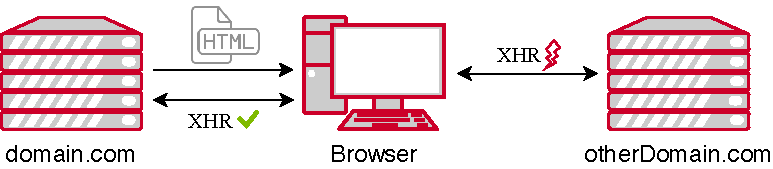
\includegraphics{gfx/SOP}
	\caption{Veranschaulichung der \textit{Same-Origin Policy}}
	\label{fig:technologies:prog:sop}
\end{figure}
Insbesondere bei modernen Webseiten ist aber genau das gewünscht, damit Webseiten von einer Domain Zugriff auf \acsp{API} anderer Domains bekommen können. Hierfür wurde das sogenannte \acf{CORS} entwickelt. In Abbildung \ref{fig:technologies:prog:cors} ist (vereinfacht) schematisch dargestellt wie mit dieser Technik Ressourcen anderer Domains angefragt werden können. Dabei wird zunächst ein \textit{Preflight Request} an einen Server geschickt, um herauszufinden, ob der Zugriff auf dessen Ressourcen möglich ist und welche Optionen (GET, POST, DELETE, etc.) unterstützt werden. Je nachdem, wie der Server konfiguriert ist, schickt er mit einer \textit{Preflight Response} einen \acs{HTTP}-Header \textit{Access-Control-Allow-Origin}, über den einer, mehreren oder allen andern Domains (bzw. deren Skripten) erlaubt wird, auf \textit{otherDomain.com} zuzugreifen. Außerdem kann über \textit{Access-Control-Allow-Methods} eingeschränkt werden, welche Operationen möglich sind. Entsprechend dieser Informationen verwirft der Browser die Anfrage oder kann sie ausführen, um dann die eigentliche Antwort zu erhalten. Dabei muss diese Technik offensichtlich vom Browser implementiert werden\cite{CORSiA}.

Bei ein paar der Ressourcen, die für diese Arbeit verwendet werden sollten, war aber genau diese serverseite Konfiguration nicht gegeben. Um diese dennoch nutzen zu können, wurde ein externer Proxy-Server (https://cors-anywhere.herokuapp.com) genutzt, welcher genau für solche Zwecke eingerichtet wurde. Um an Daten zu gelangen, deren Quelle \acs{CORS} nicht unterstützt, werden die Anfragen also an diesen Proxy-Server geschickt, der diese an den eigentlichen Server weiterleitet und die dann erhaltene Antwort wieder zum Nutzer zurückschickt. Das hat - vor allem weil die Kontrolle über diesen Proxy-Server fehlt - ganz offensichtlich zwei entscheidende Nachteile: Zum einen sind Zugriffe auf Ressourcen, die einer Authentifizierung bedürfen, über einen solchen Proxy nicht ratsam (falls überhaupt möglich) und zum anderen ist man von dessen Verfügbarkeit abhängig, weil Teile der Webanwendung nicht nutzbar sind, wenn der Proxy-Server mal wieder überlastet ist. Ebenfalls ungünstig ist die Tatsache, dass es durch diesen Umweg länger dauert, bis die Daten beim Nutzer ankommen.

\begin{figure}[h]
\centering
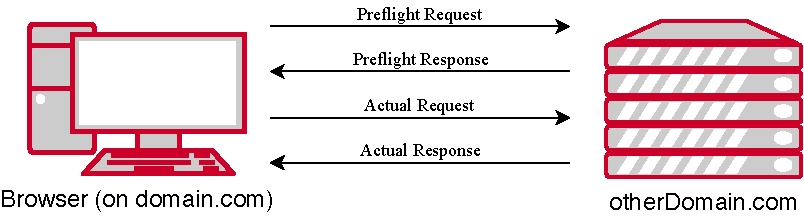
\includegraphics{gfx/CORS}
\caption[Veranschaulichung von \textit{\acf{CORS}}]{Veranschaulichung von \textit{\acf{CORS}\cite{CORSImg}}}
\label{fig:technologies:prog:cors}
\end{figure}

\subsection{JavaScript und XML}
\label{sec:prog:special:JsXml}
Viele der für dieses Projekt genutzten Daten lagen im XML-Format vor. Das ist insofern ungünstig, weil es mit JavaScript (bzw. TypeScript) wesentlich einfacher ist, \acs{JSON}-Daten zu verarbeiten: Schon der Name verrät, dass der Aufbau solcher Daten der JavaScript-Objekt-Syntax entspricht. Mit Hilfe eines Parsers, der Teil von JavaScript ist, können mit solche Daten automatisch JavaScript-Objekte erzeugt werden, die dann ganz einfach weiterverarbeitet werden können - in der Regel um das DOM um weitere Informationen zu ergänzen. Darauf bauen im Prinzip alle Frontend-Frameworks auf; bei Angular ist beispielsweise gar nicht erforderlich, den Parser selbst aufzurufen. Stattdessen definiert man vor dem Abschicken eines Requests über den \acs{HTTP}-Client, Daten welchen Typs man erwartet und das Parsen geschieht dann automatisch (vgl. Zeile 10 aus Beispiel \ref{Observables}).

Auch wenn es zwar prinzipiell möglich ist, mittels JavaScript XML-Elemente in das DOM einzubinden, lässt sich bei den meisten Frontend-Frameworks wesentlich besser mit JavaScript-Objekten arbeiten. Also mussten alle Daten, die nicht im \acs{JSON}-Format verfügbar sind, manuell aus der \acs{XML}-Struktur extrapoliert und daraus JavaScript-Objekte generiert werden. Es wäre prinzipiell möglich, einen generischen Parser zu schreiben, der aus einem \acs{XML}-String stur ein äquivalentes JavaScript-Objekt erzeug (es gibt auch Libraries Dritter, die genau das tun), da aber viele Daten in unvorteilhaften Strukturen vorliegen, wurde das Parsen für jede Datenquelle individuell implementiert. Damit konnten Objekte modelliert werden, die zur Weiterverarbeitung besser geeignet sind. Anhand des Nachrichtenmoduls wird diese Vorgehensweise einmalig erklärt und für aller weiteren Fälle ausgelassen. Dort wird dann nur noch erklärt, welche Klassen oder Interfaces zur Strukturierung der Daten modelliert wurden.

\section{Die eigentliche Programmierung}

\subsection{Vorbereitungen}
\label{sec:prog:preliminiaries}
Als erstes werden die \textit{NodeJS}-Serverumgebung sowie das Paketverwaltungssystem \textit{npm} installiert. Mit letzterem wird dann das Befehlszeileninterface von Angular (siehe Kapitel ref{sec:technologies:angular:cli}) installiert. Mit diesem wird als nächstes über den Befehl \textit{ng new Studierendenportal} ein neues Projekt mit dem Titel ``Studierendenportal`` erstellt. Dabei werden automatisch weitere Pakete installiert, welche für die Entwicklung notwendig sind - beispielsweise TypeScript (vgl. Kapitel \ref{sec:technologies:ts}). Ist dieser Vorgang abgeschlossen befindet sich in dem Ordner eine im Prinzip funktionsfähige Angular-Web-App bestehend aus einem \textit{AppModule} und einem \textit{AppComponent}. Bezogen auf den Ordner, in dem das Projekt erstellt wurde, befinden sich diese im Verzeichnis \texttt{/src/app/}, wo auch alle weiteren Dateien durch das \acs{CLI} erstellt werden. Im Verzeichnis \texttt{/src/} befinden sich zum die Index.html-Datei, ein globales Stylesheet,  ein Icon für Lesezeichen sowie ein Verzeichnis \texttt{/assets/} für andere Bilder. Sowohl im Wurzelverzeichnis als auch in \texttt{/src/} werden außerdem noch verschiedene Konfigurationsdateien erstellt. Die hauptsächliche Programmierung findet aber in \texttt{/src/app/} statt. Im Folgenden beziehen sich daher alle Angaben -  falls nicht ausdrücklich anders angegeben - auf diesen Ordner als Wurzel. Der gesamte Quellcode kann auf der beigelegten CD eingesehen werden. Außerdem kann eine funktionierende Version auf \href{http://portal.web-preview.jgulab.net/}{http://portal.web-preview.jgulab.net/} (nur erreichbar innerhalb des Universitätsnetzwerks) abgerufen werden.

\subsection{Das Grundgerüst der Anwendung}
\label{sec:prog:appmodule}
Wie bereits in Kapitel \ref{sec:technologies:angular:module} beschrieben, stellt das \textit{AppModule} - implementiert in der Datei \texttt{app.module.ts} - den Kern der ganzen Anwendung dar.  Beispiel \ref{appmodule.ts} stellt einen Ausschnitt aus \texttt{app.module.ts} dar. Da das \textit{Routing} in ein eigenes Modul ausgelagert wurde, werden dort auch alle Module, welche die eigentlichen Inhalte umfassen, importiert. Somit geschieht der Import dieser Module ins \textit{Root Module} indirekt über den Import des \textit{Router Modules}. Hierbei bedeutet ``importieren``, dass das bzw. die Modul(e) zum \textit{imports}-Array hinzugefügt werden (vgl. ab Zeile 8, \ref{appmodule.ts}). Im \textit{AppModule} müssen also nur noch die Module importiert werden, die für zusätzliche Funktionen zuständig sind. Dazu zählen beispielsweise die Module für die Authentifizierung, für den Service Worker, aber auch grundlegende Module für die Interaktion mit dem Browser oder dem \acs{DOM}.

Da an verschiedenen Stellen SVG-Icons genutzt werden sollen und es zu umständlich und zu unübersichtlich wäre, deren Quellcode an den entsprechenden Stellen direkt ins Template einzusetzen, müssen diese ebenfalls hier eingebunden werden, damit in den Templates ein Verweise auf ein solches Icon gesetzt werden kann. Während des \textit{Build}-Prozesses wird die eigentliche Graphik in das Template eingesetzt. Bei der Verwaltung der Icons wurde sich der \textit{Icon Registry} des Material Design-Pakets bedient, weil auch die Einbindung der Icons über dieses Paket umgesetzt wird. Ab Zeile 20 aus wird gezeigt, wie das geht, wobei auf gleiche Weise mehrere SVG-Icons registriert werden können; der Aufruf von \texttt{addScgIcon} kann konkateniert werden. Alternativ wäre es auch möglich, alle verwendeten SVG-Icons einer Datei quasi als \textit{Spritesheet} zusammenzufassen und diese dann zu inkludieren.

\begin{lstlisting}[float,floatplacement=h, style=htmlcssjs, caption={Ausschnitt aus \texttt{app.module.ts}}, label={appmodule.ts}]
// Importe anderer Module, Komponenten oder Services
/*...*/
@NgModule({
  declarations: [
    AppComponent,
    IndexComponent
  ],
  imports: [
	/*...*/	
    AppRoutingModule,
    CoreModule,
    MaterialModule,
    OAuthModule.forRoot(),
    ServiceWorkerModule.register('ngsw-worker.js', {enabled: environment.production})
  ],
  providers: [],
  bootstrap: [AppComponent]
})
export class AppModule {
  constructor(iconRegistry: MatIconRegistry, sanitizer: DomSanitizer) {
    iconRegistry.addSvgIcon('home',
      sanitizer.bypassSecurityTrustResourceUrl('assets/icons/home.svg'));
}
\end{lstlisting}

Weiterhin wichtig ist die Deklaration der Komponenten \textit{AppComponent} und \textit{IndexComponent} (ab Zeile 4). Das Template ersterer stellt das Grundgerüst der ganzen Web-App dar, befindet sich in der Datei \texttt{app.component.html} und wird in Ausschnitt \ref{app.component.html} wiedergegeben. Dieses Template zeigt, wie mit \textit{Angular Material} eine Seite mit einer Toolbar und einer ``responsiven``, seitlichen Navigation erstellt wird und setzt sich zunächst aus drei Bausteinen zusammen: einer Kopfleiste, in der der Titel der aktuell angezeigten Komponenten stehen soll (Zeile 3), einem Menü als Seitenbereich, in dem Links zu allen Bereichen aufgelistet sind (ab Zeile 9) und einem Container für den eigentlichen Inhalt der Seite (ab Zeile 20). Das einzige Kindelement des Inhaltscontainers ist dabei das in Kapitel \ref{sec:technologies:angular:routing} beschriebene \texttt{router-outlet}-Element, welches für die Nutzung des Routers notwendig ist. Außerdem wird mittels Event Binding erreicht, dass das Navigationsmenü geschlossen wird, wenn ein Link aus diesem Menü angeklickt wird (Zeile 10).

Besonders auffällig sind die vielen Tags, bei denen es sich offensichtlich nicht um Standard-\acs{HTML}-Elemente handelt. Stattdessen sind es alles Komponenten aus dem Material-Design-Paket. Das Element \texttt{mat-icon} ist eine solche und weil zuvor der \textit{Icon Registry} ein SVG-Icon mit dem Namen ``home`` hinzugefügt wurde, kann wie in Zeile 12 angegeben eben jene Graphik in ein Template eingebunden werden. Bei Tags und Attributes, die mit dem Präfix ``mat`` beginnen, handelt es sich um Komponenten bzw. Direktiven aus dem \textit{Angular Material}-Paket und in den folgenden Kapiteln werden noch mehr davon vorgestellt.

Die Komponente \textit{IndexComponent} beinhaltet die Startseite, welche im Grunde die gleichen Links wie das Navigationsmenü beinhaltet, nur sind sie als Karten dargestellt, in welchen kurz der Inhalt des Moduls beschrieben ist. Abbildung \ref{fig:layout1} zeigt, wie das Grundgerüst der Web-App auf einem Mobilgerät aussieht, wenn diese Startseite aufgerufen wird, und Abbildung \ref{fig:layout2} zeigt das geöffnete Menü, welches ein- und ausgeblendet wird, wenn man auf den Button oben links klickt.

\begin{lstlisting}[float, floatplacement=h, style=htmlcssjs, caption={Ausschnitt aus \texttt{app.component.hmtl} (Quelle: \href{https://material.angular.io/components/sidenav/examples}{https://material.angular.io/components/sidenav/examples})}, label={app.component.html}]
<div class="page-container">
  <!-- toolbar with heading -->
  <mat-toolbar color="primary" class="mat-elevation-z3">
    <!-- Kopfbereich -->
    <button mat-icon-button (click)="snav.toggle()" aria-label="Menü öffnen">
    <h1 id="page-title">{{title}}</h1>
  </mat-toolbar>
  <mat-sidenav-container class="mat-sidenav-container" >
    <!-- navigation menu -->
    <mat-sidenav #snav mode="over" (click)="snav.toggle()" role="navigation">
      <mat-nav-list>
        <a mat-list-item routerLink="/">
          <mat-icon svgIcon="home" color="primary" class="nav-icon"></mat-icon>
          Start
        </a>
	  <!-- ... -->
	  </mat-nav-list>
	</mat-sidenav>
    <!-- wrapper for page content -->
    <mat-sidenav-content role="main">
      <router-outlet></router-outlet>
      <!-- page content inserted from router -->
    </mat-sidenav-content>
  </mat-sidenav-container>
</div>
\end{lstlisting}

\begin{figure}
\begin{subfigure}{.5\textwidth}
  \centering
  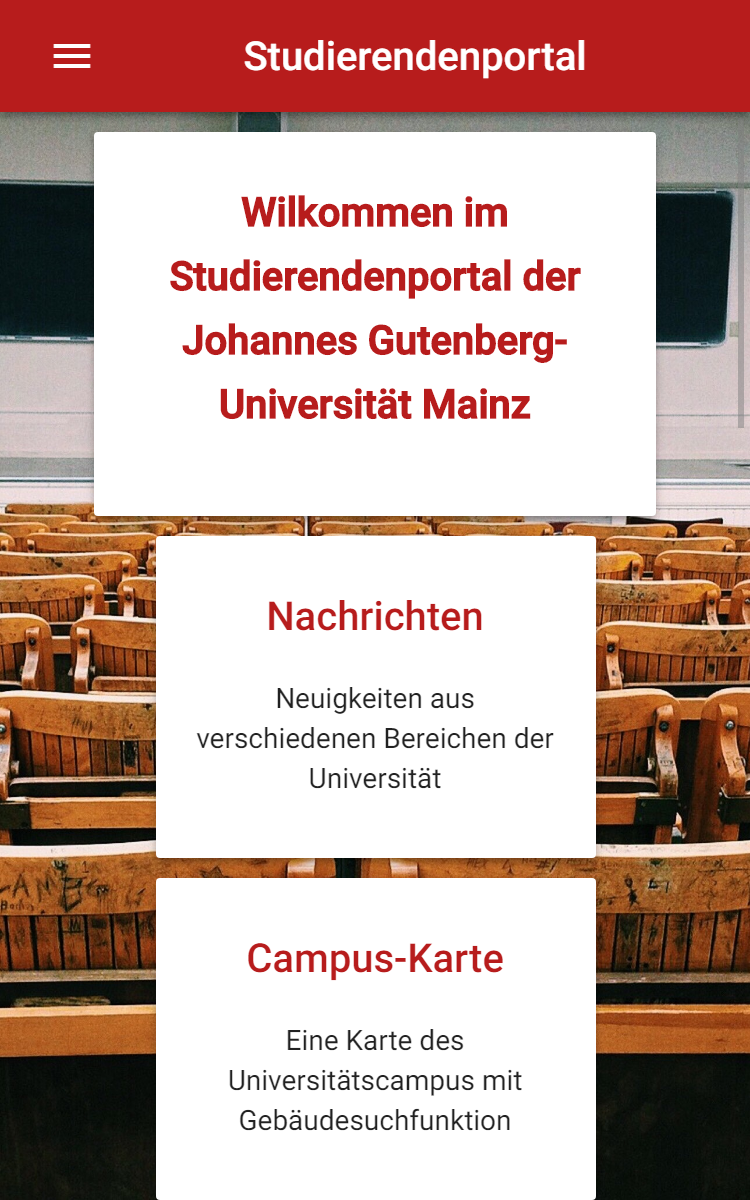
\includegraphics[width=.8\linewidth]{gfx/Layout(1)}
  \caption{normale Ansicht}
  \label{fig:layout1}
\end{subfigure}%
\begin{subfigure}{.5\textwidth}
  \centering
  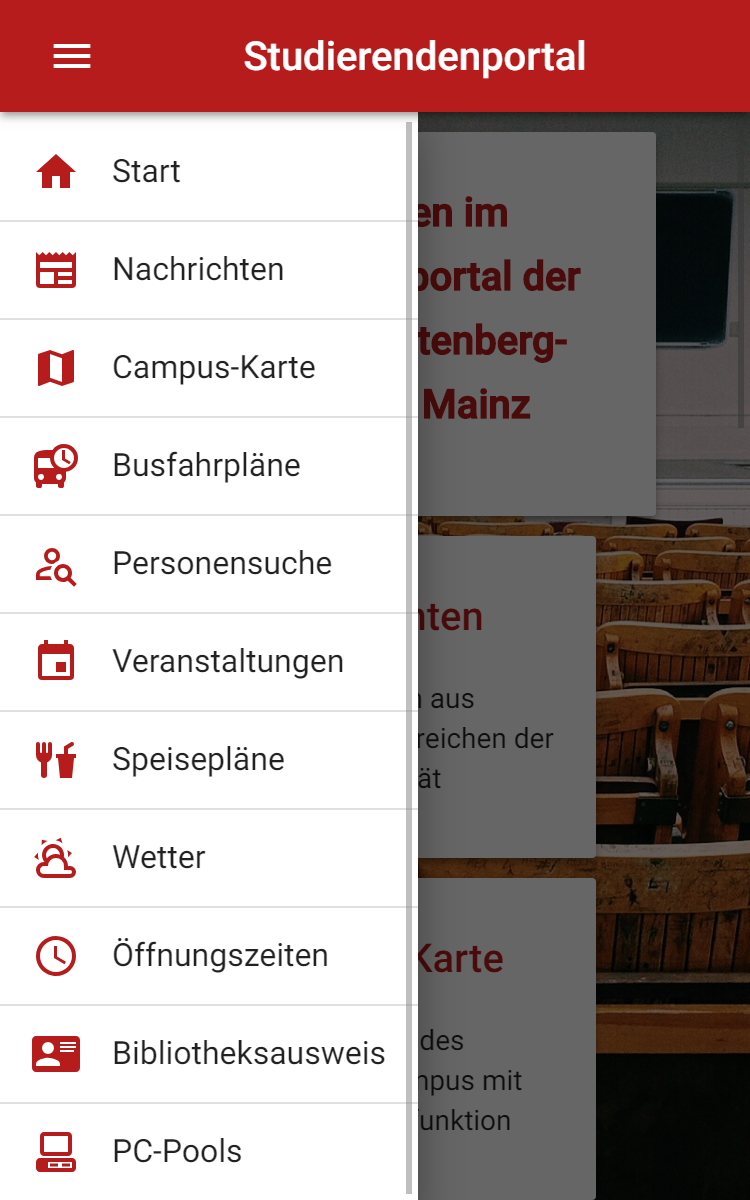
\includegraphics[width=.8\linewidth]{gfx/Layout(2)}
  \caption{mit geöffnetem Menü}
  \label{fig:layout2}
\end{subfigure}
\caption{Grundgerüst der Web-App}
\label{fig:layout}
\end{figure}

\subsection{Spezielle Module und Services}
\label{sec:prog:modules}

\subsubsection{RoutingModule}
\label{sec:prog:modules:routing}
Wie angedeutet wurde das Routing der Übersicht halber in eigenes Modul ausgelagert. Dabei wurde das \textit{Lazy Loading} außer Kraft gesetzt (vgl. Kapitel \ref{sec:technologies:angular:routing}), sodass alle Module auf einmal geladen werden. Es wäre eigentlich gar nicht zwingend notwendig gewesen, alle Inhalte in eigene Module zu unterteilen, der Übersichtlichkeit halber und weil bei zukünftigen Erweiterungen den Modulen eventuell weitere Komponenten hinzugefügt werden sollen, wurde es trotzdem getan.

\subsubsection{CoreModule}
\label{sec:prog:modules:core}
Über dieses Modul werden alle in diesem Projekt implementierten Services eingebunden. Wie beim \textit{Routing} wäre es hier ebenfalls möglich gewesen, die Services im \textit{AppModule} direkt einzubinden und auch hier wurde dies vor allem zugunsten einer besseren Übersicht nicht getan.
Zu finden ist dieses Modul in der Datei \texttt{/core/core.module.ts}. Es sei hier noch erwähnt, dass das Einbinden von Services auf globaler Ebene - was hier durch dieses Modul geschieht - bei Nutztung von \textit{Lazy Loading} wichtig ist, da auf Komponenten-Ebene eingebundene Services in nachgeladenen Modulen nicht genutzt werden können. Wird ein Service außerhalb eines Moduls nicht benötigt ist das aber unwichtig\cite{CoreModule}.

\subsubsection{MaterialModule}
\label{sec:prog:modules:material}
Es wurde bereits mehrfach erwähnt, dass das Material Design-Paket von Angular verwendet wird, um die Webseite zu gestalten. Dabei befindet sich (fast) jede Komponente dieses Pakets in einem eigenen Modul. Die meisten Komponenten dieser Web-App verwenden mehrere dieser Design-Komponenten und damit müssten alle Module der Design-Komponenten in den Modulen der eigentlichen Komponenten importiert werden. Daher wurde hier ebenfalls für eine bessere Übersicht ein weiteres Modul eingeführt, das alle benötigen Module des Design-Pakets importiert und damit bündelt. Folglich muss in den Modulen, deren zugehörige Komponenten diese Design-Komponenten verwenden, nur dieses eine Modul importiert werden. Dieses Module befindet sich in \texttt{/material/material.module.ts}.

\subsubsection{ToolbarService}
\label{sec:prog:modules:toolbar}
Bei der Erläuterung des Templates der Wurzelkomponente in Kapitel \ref{sec:prog:appmodule} wurde erklärt, dass sich der Titel im Kopfbereich der Seite (also in der Toolbar, Ausschnitt \ref{app.component.html}, Zeile 5) ändern soll, wenn zwischen den einzelnen Seiten (d.h.Komponenten) gewechselt wird. Um das umzusetzen wurde der \textit{ToolbarService} (\texttt{toolbar.service.ts}) implementiert. Dieser ist in Ausschnitt \ref{ToolbarService} wiedergegeben. In jeder Komponente wird in der jeweiligen \texttt{onInit}-Methode die Funktion \texttt{setToolbarTitle} des ToolbarService aufgerufen und der Titel der Komponente übergeben. Dieser Titel wird gleichzeitig an den TitleService, der von Angular selbst bereitgestellt wird, übergeben und somit der Seitentitel, also Beschriftung des Browser-Fensters, geändert. Im \texttt{AppComponent} wird ein Subscriber für den \textit{EventEmitter} des ToolbarService implementiert, in dem der übergebene Titel als Titel der Toolbar gespeichert wird. Ausschnitt \ref{app.component.ts} zeigt diesen Subscriber. Weil sich durch den Subscriber die Variable \texttt{title} der AppComponent ändert, ändert sich mittels \textit{Data Binding} auch der Titel der Toolbar (vgl. Ausschnitt \ref{app.component.html}, Zeile 6).

\begin{lstlisting}[float, floatplacement=h, style=htmlcssjs, caption={Ausschnitt aus \texttt{ToolBarService}}, label={ToolbarService}]
@Output() fire: EventEmitter<any> = new EventEmitter<any>();
constructor() {  }

setToolbarTitle(title: string) {
  this.fire.emit(title);
}

getEmittedValue() { return this.fire; }
\end{lstlisting}

\begin{lstlisting}[float, floatplacement=h, style=htmlcssjs, caption={``Abonnieren`` des \texttt{ToolbarService} im  \texttt{AppComponent}}, label={app.component.ts}]
export class AppComponent implements OnInit {
  title = '';
  subscription: EventListener;
  /*...*/
  ngOnInit() {
    this.subscription = this.toolbarService.getEmittedValue()
      .subscribe(title => {
        this.title = title;
      });
  }
  /*...*/
}
\end{lstlisting}

\section{Die eigentlichen Inhalte}
\label{sec:prog:components}
In dem meisten Fällen ist das Vorgehen immer das gleiche: Bei Initialisierung einer Komponente werden über einen Service Daten angefragt, die anschließend unter Umständen vom Service geparst werden müssen, bevor sie dann in das Template der Komponente eingesetzt werden. Lediglich beim Karten-Modul und bei der Personensuche ist das Vorgehen (leicht) abweichend. Zur Verarbeitung der Daten wurden mehrere Klassen und Interfaces definiert, die sich alle im Verzeichnis \texttt{models} befinden.

\subsection{Nachrichten}
\label{sec:prog:news}
\begin{lstlisting}[float, floatplacement=h, style=htmlcssjs, caption={Ausschnitt aus dem NewsFeedService}, label={newsfeedservice}]
parseFeedFromXmlToJson(feedAsString: string, feedName: string) {
  const feedAsJson: Feed = new Feed(feedName);
  const feedAsXml = new DOMParser().parseFromString(feedAsString, 'application/xml');
  const feedItems = (feedAsXml.getElementsByTagName('item'));

  for (let index = 0; index < feedItems.length; index++) {
    const feedItem: FeedPost = new FeedPost();
    const itemAsXml = feedItems.item(index);
    const categories = item.getElementsByTagName('category');
    feedItem.title = itemAsXml.getElementsByTagName('title')[0].firstChild.nodeValue;
    /*...*/
    feedAsJson.items.push(feedItem);
  }
  this.sortItems(feedAsJson);
  this.feedsAsJSON.push(feedAsJson);
}
\end{lstlisting}
Der Service dieses Moduls\footnote{\texttt{/news-feed/news-feed.service.ts}} enthält vier Funktionen, von denen die komplexeste, welche für das Parsen zuständig ist, in Ausschnitt \ref{newsfeedservice} auszugsweise wiedergegeben wird. In dieser wird zunächst ein \texttt{Feed}-Objekt\footnote{\texttt{/models/feed.ts}} erzeugt, welches einen Namen hat und eine Liste von \texttt{FeedPost}-Objekten\footnote{\texttt{/models/feedPost.ts}} enthält. Diese wiederum setzen sich zusammen aus einem Titel, einer Beschreibung, einem Link zum eigentlichen Artikel, einem Veröffentlichungsdatum sowie einer Reihe von Kategorien, zu denen der jeweilige Post gehört.

Bevor die eigentlichen Posts des RSS-Feeds geparst werden, muss aus dem übergebenen \acs{XML}-String ein \acs{DOM}-Objekt erzeugt werden und dann wie in Zeile 4 die Liste der Posts (ausgezeichnet durch einen \textit{item}-Tag) abgefragt werden. Anschließend wird über diese Liste iteriert, alle Eigenschaften des jeweiligen Posts abgefragt und diese im erzeugten \texttt{feedPost}-Objekt gespeichert. Wie das Abfragen der Attribute funktioniert, ist in Zeile 10 dargestellt. Weil mit \texttt{getElementsByTagName} immer eine Liste vom Typ \texttt{NodeList} zurückgegeben wird und ein Post genau einen Titel hat, wird ebenjener über den Index '0' erreicht. Um den eigentlichen Inhalte \texttt{item}-Elements zu erhalten, ist der Aufruf \texttt{.firstChild.nodeValue} notwendig, was am Aufbau eines solchen \textit{Node}-Elements liegt.

Mit den Kategorien des Post wird analog in einer weiteren Schleife (hier nicht gezeigt) verfahren und diese Kategorien dann dem Post hinzugefügt. Als nächstes werden die Einträge des Feeds chronologisch sortiert, bevor dieser in der Liste der Feeds gespeichert wird.

\begin{lstlisting}[float, floatplacement=h, style=htmlcssjs, caption={Abfragen der Feeds im \texttt{NewsFeedComponent}}, label={NewsFeedComponent}]
getFeeds() {
  this.feedSources = this.feedService.getFeedSources();
  if ((this.feeds = this.feedService.feedsAsJSON).length === 0) {
    this.feedSources.forEach(src => {
      this.feedService.getNewsFromFeed(src.url).subscribe(feed => {
        this.feedService.parseFeedFromXmlToJson(feed, src.name);
      });
    });
  }
}
\end{lstlisting}
Hier nicht gezeigt sind die Funktionen zum Sortieren, zum Abfragen des Feeds vom Server sowie zum Abfragen der Liste der Feed-Quellen. Diese Liste befindet sich in einer eigenen Datei\footnote{\texttt{/news-feed/RssFeeds.json}} und enthält eine Reihe von Objekten, die sich aus einem Namen sowie der URL des Feeds zusammensetzen. Auf diese Weise können sehr einfach weitere RSS-Feeds eingebunden werden. Das Abfragen der Daten durch den \acs{HTTP}-Client unterscheidet sich hier insofern von dem Aufruf in Beispiel \ref{Observables}, als keine Klasse, Instanzen derer man erwartet, angeben wird, sondern dem \texttt{get}-Aufruf die Option ``\texttt{\{responseType: \textquotesingle text\textquotesingle \}}`` mitgegeben wird. Damit wird deklariert, dass kein(e) \acs{JSON}-Objekt(e) sondern nur einfacher Text - also im Prinzip ein String - erwartet wird. Außerdem wird im Aufruf der eigentlichen \acs{URL} der Ressource die \acs{URL} des Proxy-Servers vorangestellt. Anhand des Ausschnitts \ref{BusScheduleService} in Kapitel \ref{sec:prog:bus} wird dies genauer erklärt.

Bei der Initialisierung der \texttt{NewsFeedComponent}\footnote{\texttt{/news-feed/news-feed-component/news-feed.component.ts}} werden zwei Funktionen aufgerufen: In einer wird  der Titel der Seite sowie der Toolbar (vgl \ref{sec:prog:modules:toolbar}) geändert und in der anderen das Abfragen der Feeds durchgeführt. In letzterer - wiedergegeben in Ausschnitt \ref{NewsFeedComponent} - werden zunächst die Quellen abgefragt und danach geprüft, ob im Service bereits die Feeds als \acs{JSON} gespeichert sind - also ob die Liste derer leer ist oder nicht (Zeile 3). Allerdings wird hier kein Objekt ``kopiert``, sondern eine Referenz gesetzt, sodass, wenn beim Parsen im Service die Liste der Feeds aktualisiert wird (vgl. Ausschnitt \ref{newsfeedservice}, Zeile 5), dies auch automatisch mit der Liste in der Komponente geschieht. Beim Aufruf der Methode zum Übersetzten in Zeile 6 findet daher keine Rückgabe statt.

Weil durch Navigieren zwischen Seiten über das Menü die Komponenten mitsamt ihrer Daten immer ``zerstört`` und neu ``konstruiert`` werden, müssten jedes mal, wenn eine Komponente erzeugt wird, die Daten neu vom Server angefragt und anschließend geparst werden. Wenn später der Service Worker hinzugefügt wird, können zwar die \acs{XML}-Daten aus dem Cache bezogen werden, um etwas Zeit zu sparen, trotzdem müssen sie dann noch in \acs{JSON}-Objekte übersetzt werden. Da der Service (bzw. alle Services, das gleiche Prinzip gilt auch für die anderen Module) global existiert, gehen die Daten  - einmal übersetzt und im Service gespeichert - nicht verloren, wenn zu einer anderen Komponente und zurück navigiert wird. 

\begin{lstlisting}[float, floatplacement=h, style=htmlcssjs, caption={Ausschnitt des NewsFeed-Templates}, label={news-feed.component.html}]
<mat-tab *ngFor="let feed of feeds" label="{{feed.name}}">
  <div class="output">
    <mat-card *ngFor="let item of feed.items" (click)="openLinkForItem(item)" class="mat-elevation-z3">
      <mat-card-header>
        <mat-card-title>
          <h3>{{ item.title }}</h3>
        </mat-card-title>
        <mat-card-subtitle>{{item.pubDate | date: 'dd.MM.yyyy' }}</mat-card-subtitle>
      </mat-card-header>
      <mat-card-content [innerHtml]="item.description"></mat-card-content>
      <mat-card-footer>
		<!--list of  -->
      </mat-card-footer>
    </mat-card>
  </div>
</mat-tab>
\end{lstlisting}

Das Code-Beispiel \ref{news-feed.component.html} zeigt einen Ausschnitt aus dem Template dieser Komponente\footnote{\texttt{/news-feed/news-feed-component/news-feed.component.html}}. In einem Registerkartenlayout (\texttt{mat-tab}) werden die Posts als Liste von Karten (\texttt{mat-card}) angezeigt, wobei im Kopfbereich der Titel sowie das Veröffentlichungsdatum stehen, im Inhaltsbereich die Beschreibung (also eine Zusammenfassung) eingefügt wird und im Fußbereich die Kategorien aufgelistet sind. Klickt man eine solche Karte an, wir der Link des Beitrags geöffnet, wobei dies über eine Funktion - also mittels \textit{Event Binding} - geschieht (Zeile 3), in der geprüft wird, ob ein Mobilgeräte verwendet wird und in diesem Fall eine Bestätigung angefordert wird, damit beim Scrollen durch die Meldungen nicht unbeabsichtigt ein Link geöffnet wird.

Abbilding \ref{fig:news} zeigt, wie der Feed der als Karten dargestellten Meldungen auf einem Smartphone aussieht. Zunächst einmal sieht man, dass der Titel der Toolbar am oberen Bildrand geändert wurde. Darunter sieht man die Tabs (Registerkarten), mit denen zwischen den Quellen gewechselt werden kann und danach sind die Posts des jeweiligen Feeds aufgelistet.

\begin{figure}
\begin{subfigure}{.5\textwidth}
  \centering
  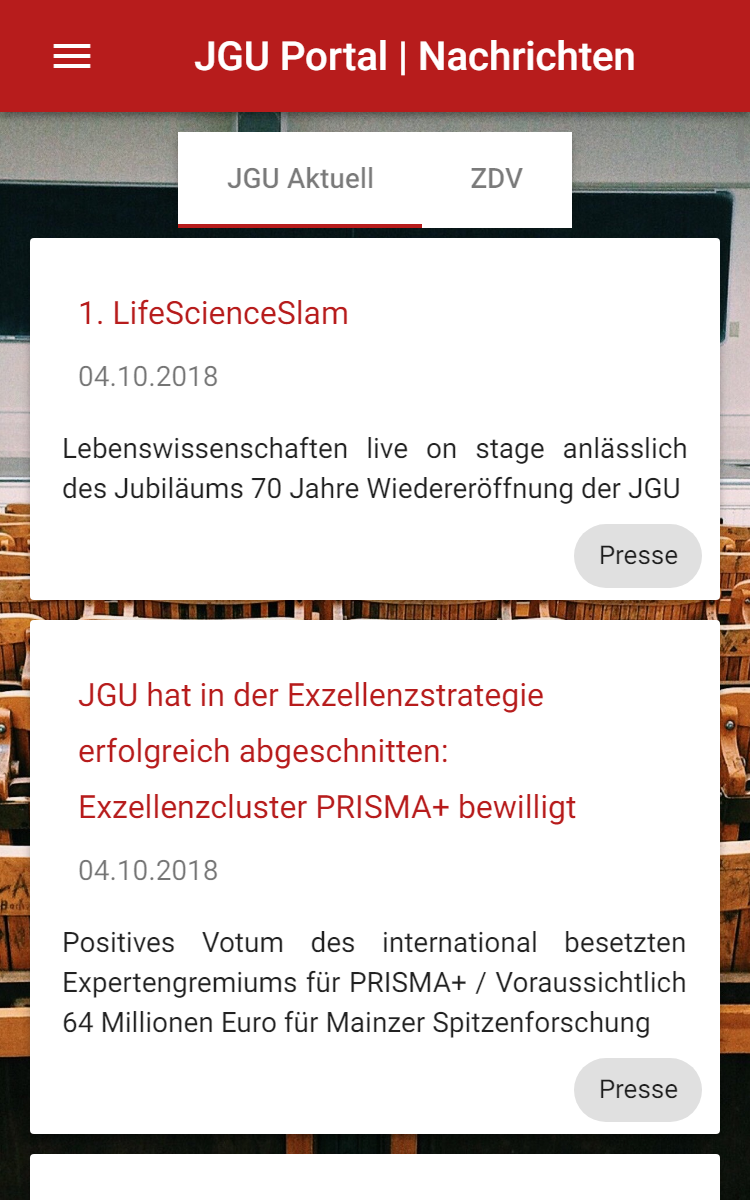
\includegraphics[width=.8\linewidth]{gfx/NewsFeed}
  \caption{Das Nachrichtenmodul}
  \label{fig:news}
\end{subfigure}%
\begin{subfigure}{.5\textwidth}
  \centering
  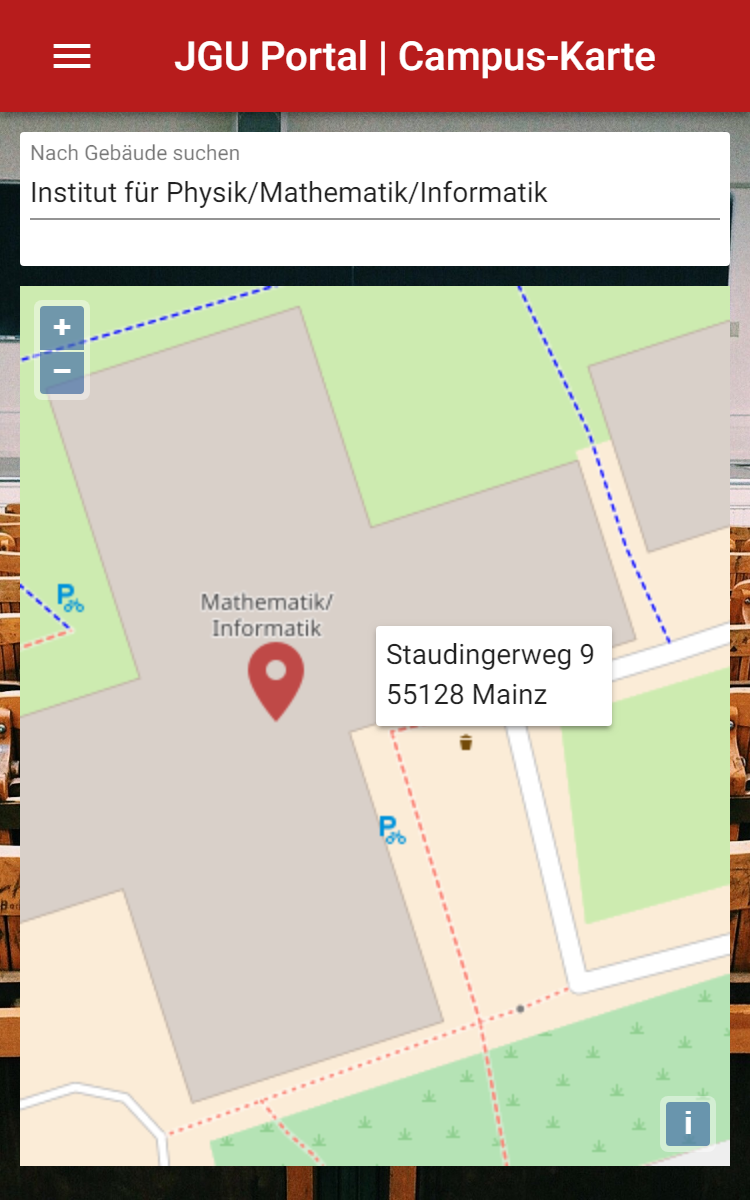
\includegraphics[width=.8\linewidth]{gfx/Map}
  \caption{Das Kartenmodul}
  \label{fig:map}
\end{subfigure}
\caption{Das Nachrichten - und das Kartenmodul}
\label{fig:news+map}
\end{figure}

\subsection{Campus-Karte}
\label{sec:prog:map}
Damit in diesem Modul die Gebäude auf der Karte angezeigt werden können, muss bei Initialisierung der Komponente zunächst ein Liste ebendieser bezogen werden. Da diesen Daten im \acs{JSON}-Format vorliegen, sieht die \texttt{getBuildingsList}-Methode des MapService\footnote{\texttt{/map/map.service.ts}} im Prinzip genauso aus wie in Beispiel \ref{Observables}, nur das ein Array von \texttt{Building}-Objekten erwartet wird. Ein solches \texttt{Building}-Objekt\footnote{\texttt{/models/building.ts}} enthält: einen Namen, einen ``Nicknamen``, eine Adresse, und ein \texttt{Coordinate}-Objekt\footnote{\texttt{/models/coordinate.ts}}, welches wiederum aus Längen- und Breitengrad besteht. Dabei könnte man die Daten im Service speichern, sobald der Service Worker hinzugefügt wird, speichert dieser die Ressource ohnehin im Cache, sodass dies an dieser Stelle nicht notwendig ist.

\begin{lstlisting}[float, floatplacement=h, style=htmlcssjs, caption={Auszug aus MapComponent}, label={FilterBuildings}]
private getBuildings() {
  this.mapService.getBuildingsList()
    .subscribe(res => {
      this.buildings = res;
      this.filteredBuildings = this.ctrl.valueChanges
        .pipe(
          startWith(''),
          map(buildingName => this.filterBuildings(buildingName))
        );
    });
}

private filterBuildings(name: string): Building[] {
  const filterValue = name.toLowerCase();
  return this.buildings.filter(building => {
    return building.name.toLowerCase().startsWith(filterValue)
    || (building.nickname && building.nickname.toLowerCase().startsWith(filterValue));
  });
}
\end{lstlisting}
Um die Suchfunktion mit Auto-Vervollständigung durchführen zu können, müssen in MapComponent\footnote{\texttt{\texttt{/map/map-component/map.component.ts}}} zwei Dinge geschehen: Eine Kopie der Gebäudeliste muss angelegt werden und in dieser Liste müssen diejenigen Gebäude hinterlegt werden, deren Namen mit der aktuellen Eingabe übereinstimmen. Die zwei Funktionen in Ausschnitt \ref{FilterBuildings} setzen dies um. Hierfür wird nach Empfang der Daten ein Observable (\texttt{FilteredBuildings}) initialisiert (Zeile 5), welches ein Array vom Typ \texttt{Building} ``kapselt``. Über ein \textit{FormControl}-Objekt (\texttt{ctrl}) wird diesem Observable jedes Mal durch die Pfeilfunktion in Zeile 8 eine neue Liste an Gebäuden zugewiesen, wenn eine Eingabe getätigt wird. Genauer: bei \texttt{ctrl.valueChanges} handelt es sich ebenfalls um ein Observable, dessen Zustand - also der Wert - sich ändert, wenn ein Eintrag aus der Liste der Gebäude ausgewählt wird. Der Aufruf von \texttt{startWith} ist wichtig, damit initial alle Gebäude als Drop-Down-Liste angezeigt werden. In der \texttt{filterBuildings}-Methode (Zeile 13) werden dann diejenigen Gebäude herausgesucht, deren Name oder Nickname mit dem übergebenen String beginnt.

Das Anzeigen der Karte wird in der Methode \texttt{ngAfterViewInit} implementiert, wobei diese Methode über das Interface \texttt{AfterViewInit} bereitgestellt wird und erst aufgerufen wird, wenn das Template der Komponente auch vollständig initialisiert wurde. Warum das so sein muss, lässt sich an Ausschnitt \ref{Map}. In Zeile 9 wird das Attribut \texttt{target} definiert, wobei eine ID - in diesem Fall ``map`` - angegeben wird, welche ein \acs{DOM}-Element referenziert, als dessen Kind ein \textit{Canvas}-Element erzeugt wird, auf welchem wiederum die Karte erstellt wird. Würde diese Initialisierung bereits durch die \texttt{onInit}-Methode ausgelöst, kann es sein, dass das Template noch nicht vollständig ins \acs{DOM} eingebunden wurde, sodass dort noch gar kein Element mit der ID ``map`` vorhanden ist - die Initialisierung würde also scheitern.

Neben dem \textit{target}-Attribut werden noch weitere Eigenschaften des \texttt{Map}-Objektes festgelegt: unter \texttt{layers} werden die einzelnen Schichten der Karte definiert, wobei das \texttt{TileLayer} das eigentliche Kartenmaterial enthält, welches in diesem Fall von OpenstreetMap (OSM) stammt, und mit dem \texttt{VectorLayer} Vektordaten oder - wie in diesem Fall - Bilder bzw. Icons auf der Karte angezeigt werden können. Über das Attribut \texttt{view} können initiale Position und Zoom festgelegt werden - in diesem Fall wird (in etwa) das Zentrum des Universitäts-Campus angezeigt  und so nah ``herangezoomt``, dass dessen Darstellung ungefähr den ganzen Bildschirm füllt.
\begin{lstlisting}[float, floatplacement=h, style=htmlcssjs, caption={Initialisieren der Karte}, label={Map}]
ngAfterViewInit() {
  this.myMap = new Map({
    layers: [
      new TileLayer({
        source: new OSM // Base Layer with tiles
      }),
      new VectorLayer({ source: this.markerSource })
    ],
    target: 'map',
    view: new View({
      center: fromLonLat([8.2411, 49.9923], 'EPSG:3857'),
      zoom: 16
    })
  });
  this.popupOverlay = new Overlay({
    element: this.popup.nativeElement,
    positioning: 'bottom-left',
    stopEvent: false,
    position: this.myMap.getView().getCenter()
  });
  /*...*/
  this.myMap.addOverlay(this.popupOverlay as ol.Overlay);
}
\end{lstlisting}
Hat man ein Gebäude aus der Vorschlagsliste ausgewählt, geschehen in der Funktion \texttt{centerMapAtBuilding} (hier nicht gezeigt) im Wesentlichen vier Dinge: 

\begin{itemize}
\item Die Zoom-Stufe wird erhöht.
\item Die Karte wird um das ausgewählte Gebäude zentriert.
\item Das Gebäude wird mit einem Icon markiert.
\item Ein Textfeld, welches die Adresse des Gebäudes enthält, wird neben dem Marker angezeigt.
\end{itemize}

Um das Textfeld anzuzeigen wird, wie ab Zeile 15(\ref{Map}) dargestellt, ein Overlay erzeugt und dieses dem Karten-Objekt hinzugefügt (ab Zeile 15). Hierbei wird mit \texttt{this.popup.nativeElement} ein \acs{DOM}-Element referenziert, welches als Kindelement das eigentliche Popup hat. Das zugehörige Template\footnote{\texttt{/map/map-component/map.component.html}} ist in Code-Beispiel \ref{MapTemplate} wiedergegeben, wo das Element für die Karte sowie für das Popup-Overlay samt Adresskarte ab Zeile 12 definiert werden. Während der Marker solange angezeigt wird, bis man ein anderes Gebäude ausgewählt oder zu einer anderen Seite navigiert, wird das Textfeld ausgeblendet, wenn die Zoomstufe zu niedrig ist, da dieses anderenfalls den Marker überlagern würde.  Dies geschieht,  indem dem \texttt{Map}-Objekt ein \textit{EventListener} zugweisen wird, welcher auf das 'scroll'-Event reagiert und das Attribut \texttt{showAdress} des \texttt{MapComponent} in Abhängigkeit Zommstufe auf \texttt{true} oder \texttt{false} setzt.  Mittels \textit{Attribute Binding} wird in Zeile 14 erreicht, dass - je nachdem, ob \texttt{showAddress} 'wahr' oder 'falsch' ist - die \textit{Opacity} des Elements auf '0' oder '1' gesetzt wird, wobei der Übergang mit \acs{CSS}\footnote{\texttt{/map/map-component/map.component.scss}} animiert wird. Die \texttt{*ngIf}-Direktive ist notwendig, damit die Adresskarte nicht angezeigt wird wenn (noch) kein Gebäude ausgewählt wurde.

\begin{lstlisting}[float, floatplacement=h, style=htmlcssjs, caption={Template des MapComponent}, label={MapTemplate}]
<mat-form-field class="selectForm">
  <input matInput type="text" id="searchField" name="searchField"
         [formControl]="ctrl" [matAutocomplete]="auto">
</mat-form-field>
<mat-autocomplete #auto="matAutocomplete">
  <mat-option *ngFor="let building of filteredBuildings | async" [value]="building.name"
              (onSelectionChange)="centerMapAtBuilding(building, $event)">
      {{ building.name }}
    <span *ngIf="building.nickname">({{ building.nickname }})</span>
  </mat-option>
</mat-autocomplete>
<div id="map">
  <div #popup>
    <mat-card id="address" *ngIf="focusedBuilding !== undefined" [style.opacity]="showAddress? '1':'0'" >
      {{ focusedBuilding.defaultAddress }}
    </mat-card>
  </div >
</div>
\end{lstlisting}

Vorher werden das Eingabefeld sowie die Liste der Gebäude angegeben. Auch hier wird zweimal \textit{Attribute Binding} verwendet: Zum einen um das \textit{formControl}-Objekt \texttt{ctrl} zuzuweisen und zum anderen, um das Eingabefeld mit der Autovervollständigung zu verknüpfen (Zeile 3). Anschließend werden alle Gebäude als ``Option`` gelistet. Hierbei wird die \texttt{async}-Pipe genutzt weil es sich bei \texttt{filteredBuildungs} um ein \textit{Observable} handelt; dessen Wert sich kann also jederzeit ändern und wenn das geschieht, muss die Liste neu erstellt werden.

Bei jeder Option wird hier der Name (Zeile 8) und - falls vorhanden - der \textit{Nickname} (Zeile 9) des Gebäudes angezeigt. Außerdem wird mittels \textit{Data-Binding} jeder Option der Name des jeweiligen Gebäudes als \texttt{value} zugeordnet, sodass dieser in das Eingabefeld übertragen wird, wenn man die Option auswählt. Wird ein solches Element ausgewählt, wird mittels \textit{Event Binding} (Zeile 7) die Methode zum Zentrieren etc. aufgerufen. Dabei wird neben dem ausgewählten Gebäude auch das Event übergeben. Das ist notwendig, weil bei Veränderung der Auswahl das ``selectionChange``-Event sowohl durch das ``Abwählen`` des alten Gebäudes, als auch durch Auswählen des neuen Gebäudes ausgelöst wird - also zweimal. Durch Übergabe des Events ist es möglich, zu prüfen, welches der beiden Ereignisse tatsächlich eingetreten ist. Wurde kein Gebäude ausgewählt, kann die Karte auch nicht zentriert werden und der Funktionsaufruf wird beendet.

\subsection{Busfahrpläne}
\label{sec:prog:bus}
Die Abfahrtszeiten für dieses Modul werden über die \acs{API} des Rhein-Main Verkehrsverbundes bezogen und können als \acs{JSON} angefragt werden. Für dieses Module wurden die in Abbildung \ref{fig:programming:busStops} dargestellten Klassen modelliert. Das Attribut \texttt{name} der \texttt{Departure}\footnote{\texttt{/models/departureBoard.ts}} \footnote{\texttt{/models/departure.ts}}-Klasse bezieht sich dabei auf den Namen der Bus- bzw. Straßenbahnlinie und \texttt{direction} gibt den Namen der Endhaltestelle an. Die Attribute \texttt{rtTime} und \texttt{rtDate} in derselben Klasse beziehen sich auf die derzeit erwartete Verspätung. Während die ``Abfahrtstafeln`` (\texttt{Departure}) über die \acs{API} bezogen werden müssen, sind die Bushaltestellen (\texttt{BusStop}\footnote{\texttt{/models/busStop.ts}}\footnote{\texttt{/models/coordinate.ts}}) in einer Datei lokal gespeichert\footnote{\texttt{/bus-schedule/busStops.json}}. Diese Datei wird über den \texttt{BusStopService}\footnote{\texttt{/bus-schedule/bus-schedule.service.ts}} importiert, welcher wiederum eine Methode enthält, damit diese Liste der Haltestellen in der Komponente\footnote{\texttt{/bus-schedule/bus-schedule-component/bus-schedule.component.ts}} abgefragt werden kann.
\begin{figure}[h]
\centering
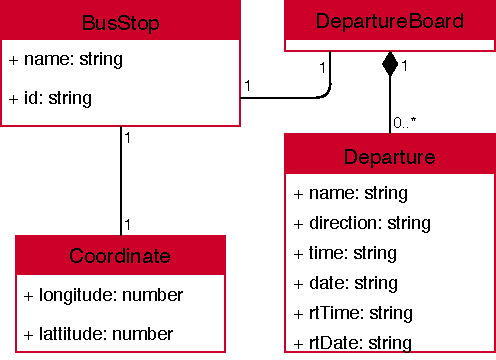
\includegraphics{gfx/BusStops}
\caption{UML-Diagramm der Klassen des Busfahrplan-Moduls}
\label{fig:programming:busStops}
\end{figure}
In dieser Komponente ist die in Ausschnitt \ref{busStopComponent} angegebene Funktion implementiert. In dieser wird zunächst die Liste der Bus- und Straßenbahnhaltestellen bezogen (Zeile 2) und dann für jede dieser Haltestellen die Abfahrtszeiten abgefragt, sodass diese bei der jeweiligen Haltestelle gespeichert werden können. 

\begin{lstlisting}[float, floatplacement=h, style=htmlcssjs, caption={Ausschnitt aus \texttt{BusStopComponent}}, label={busStopComponent}]
private initBusStops() {
  this.busStops = this.busStopService.getBusStops();
  this.busStops.forEach(busStop => {
    this.busStopService.getDepartureBoardForStation(busStop.id)
      .subscribe(departureBoard => {
        busStop.departureBoard = departureBoard;
      });
  });
}
\end{lstlisting}

Das eigentliche Abfragen ist hier etwas komplexer, da die \acs{URL} für die Anfrage aus mehreren Parametern zusammen gesetzt werden muss, wie in Ausschnitt \ref{BusScheduleService} dargestellt. Zunächst wird der \texttt{apiKey}-angegeben, ohne welchen ein Zugriff auf die RMV-API gar nicht möglich ist. Durch den Parameter \texttt{format} wird erreicht, dass die Daten als \acs{JSON} und nicht im \acs{XML}-Format übertragen werden, was der Standard wäre. Weiterhin wird mit \texttt{maxLength} festgelegt, dass höchstens die nächsten 10 Abfahrten übertragen werden. Aus diesen Parametern wird dann die eigentliche \acs{URL} zusammengesetzt. In der eigentlichen Anfrage (Zeile 6) wird dann noch die \acs{URL} des Proxy-Servers vorangestellt, sowie die ID der Bushaltestelle, deren Abfahrtstafel bezogen werden soll, angehängt.

\begin{lstlisting}[float, floatplacement=h, style=htmlcssjs, caption={Abfragen der Abfahrtstafeln im BusScheduleService}, label={BusScheduleService}]
const proxy = 'https://cors-anywhere.herokuapp.com/';
const apiKey = 'accessId=26594e9d-0888-496c-a664-5b0b888f3882';
const format = '&format=json';
const maxLength = '&maxJourneys=10';
const url = 'https://www.rmv.de/hapi/departureBoard?' + apiKey + format + maxLength;

getDepartureBoardForStation(stationID: number): Observable<DepartureBoard> {
  return this.http.get<DepartureBoard>(proxy + url + `&id=${stationID}`);
}
\end{lstlisting}
Dabei könnten die Daten - also die Abfahrtstafeln theoretisch im Service gespeichert werden, da sich die Abfahrtszeiten (oder Verspätungen) aber fast im Sekundentakt ändern, wird hier darauf verzichtet. Somit liegen immer die aktuellsten Informationen vor, wenn von dieser Komponente zu einer anderen und zurück navigiert wird. Weiterhin wäre es ebenso möglich gewesen, mittels \texttt{setInterval} die Daten regelmäßig auch dann zu aktualisieren, wenn der Nuzter auf dieser Seite verbleibt. Da so jedoch relativ schnell das Pensum der maximal erlaubten Anfragen pro Stunde bzw. pro Tag überschritten würde, wenn entsprechend viele Studierende dieses Angebot nutzen. Dementsprechend wurde auch hierauf verzichtet. Außerdem wurde aus demselben Grund davon abgesehen diese Daten über den Service Worker im Cache zu speichern.

Abbildung \ref{fig:busStops} zeigt die Ansicht der Abfahrtszeiten. Zu jeder Haltestelle gibt es ein Akkordeon-Element in dem die als nächstes an dieser Station ankommenden Busse und Straßenbahnen inklusive deren Informationen tabellarisch aufgelistet sind. Kommen in nächster Zeit keine Busse oder Straßenbahnen an, wird ``keine Abfahrten in nächster Zeit`` angezeigt.

\begin{figure}
\begin{subfigure}{.5\textwidth}
  \centering
  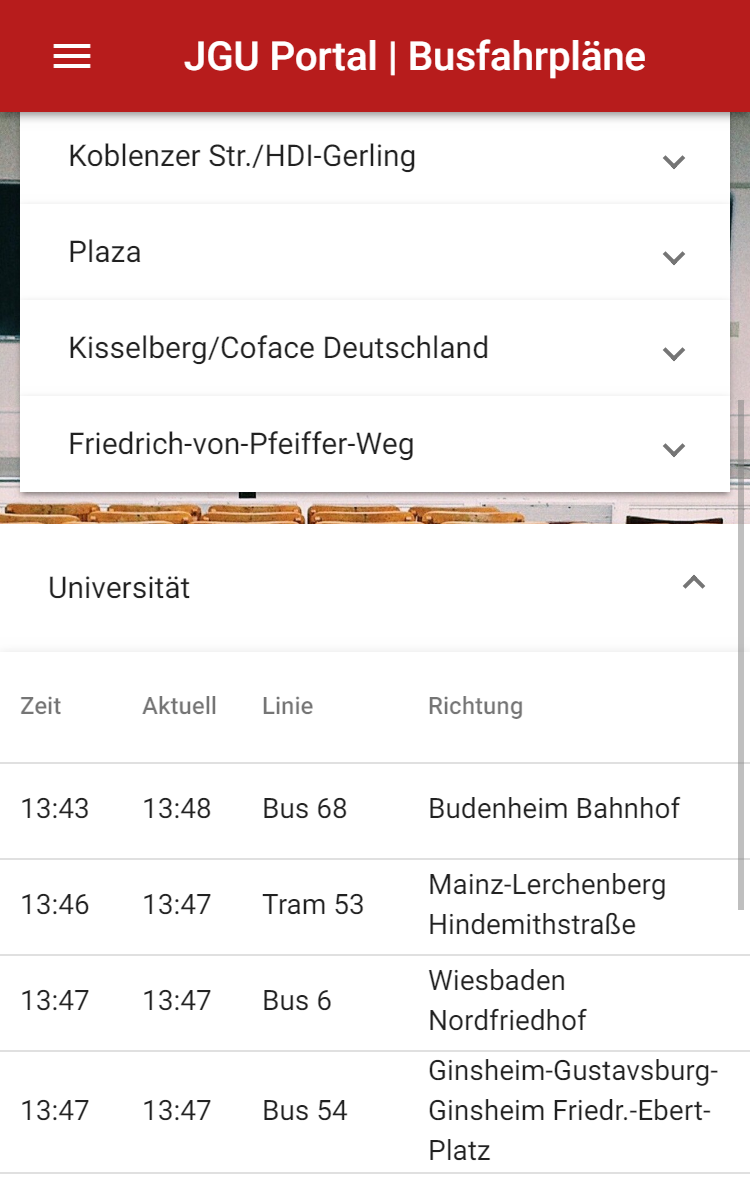
\includegraphics[width=.8\linewidth]{gfx/Busse}
  \caption{Ansicht der Busfahrpläne}
  \label{fig:busStops}
\end{subfigure}%
\begin{subfigure}{.5\textwidth}
  \centering
  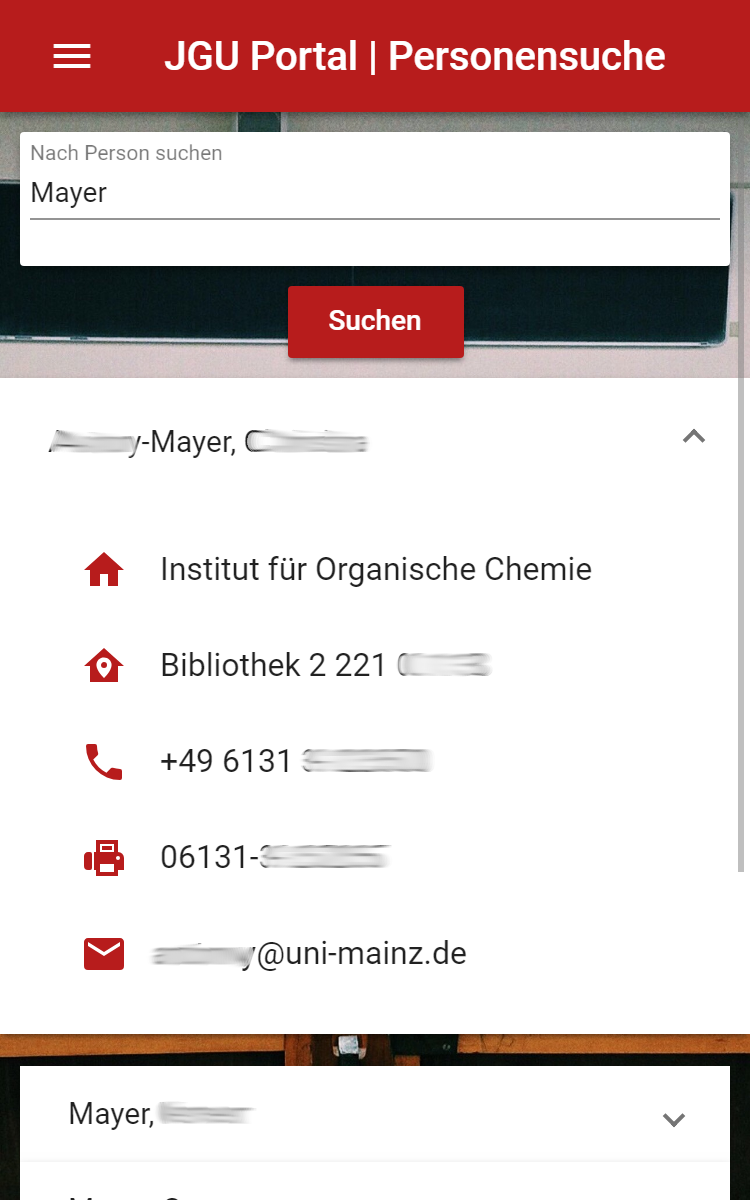
\includegraphics[width=.8\linewidth]{gfx/Personen}
  \caption{mit geöffnetem Menü}
  \label{fig:persons}
\end{subfigure}
\caption{Das Abfahrtszeiten- und das Personensuchmodul}
\label{fig:busStops+Persons}
\end{figure}
Wie eine solche Tabelle mit \textit{Angular Material} generiert werden kann, ist in dem Auszug \ref{Departures} dargestellt\footnote{\texttt{/map/map-component/map.component.html}}. Hierfür wird zunächst die Tabelle mittels \textit{Data-Binding} mit einem Datensatz verknüpft, der dargestellt werden soll. Außerdem wird für die jeweilige Station geprüft, ob Abfahrten vorhanden sind, da anderenfalls ein hier nicht gezeigtes Template (referenziert mit \texttt{noDepartures}) angezeigt wird, welches lediglich ``keine Abfahrten in nächster Zeit`` enthält (Zeile 1). Anschließend werden für jede Spalte Container definiert, in denen deren Überschrift und eine Liste der Werte, über die iteriert werden soll, angegeben wird. Außerdem wird angeben, welchen Inhalt die Zeilen dieser Spalte haben sollen (Zeile 5). In diesem Fall wird hier die Spalte der geplanten Abfahrtszeiten definiert. Da diese Information getrennt in Datum und Uhrzeit vorliegt, müssen diese Angaben konkateniert werden um eine ISO 8601-konforme Angabe zu erhalten, der dann durch die Pipe formatiert werden kann.

Mit Hilfe dieser Container werden dann die eigentlichen Zeilen der Tabelle erzeugt: In Zeile 10 wird die Kopfzeile generiert und in Zeile 11 die Inhaltszeilen. Dabei wird mit \texttt{displayedColumns} jeweils ein String-Array übergeben, in dem die Namen der Spalten die angezeigt werden sollen, aufgelistet sind. Diese Namen beziehen sich auf die zuvor definierten Container, sodass die Reihenfolge der Spalten von der Reihenfolge der Spaltennamen im Array und nicht von der der Container abhängig ist. Indem Einträge aus dem Array gelöscht oder diesem hinzugefügt werden, können Spalten ein- oder ausgeblendet werden. Dementsprechend müssen auch nicht alle Container referenziert werden; nicht genutzte Container sind dann nicht Teil des \acsp{DOM}.

\begin{lstlisting}[float, floatplacement=h, style=htmlcssjs, caption={Tabelle der Abfahrtszeiten}, label={Departures}]
<table mat-table *ngIf="station.departureBoard.Departure !== undefined; else noDepartures"
             [dataSource]="station.departureBoard.Departure" class="mat-elevation-z3">
  <ng-container matColumnDef="Abfahrt (geplant)">
    <th mat-header-cell *matHeaderCellDef>Zeit</th>
    <td mat-cell *matCellDef="let departure">
      {{ departure.date + 'T' + departure.time | date:'HH:mm'}}
    </td>
  </ng-container>
    <!-- ... -->
  <tr mat-header-row *matHeaderRowDef="displayedColumns"></tr>
  <tr mat-row *matRowDef="let row; columns: displayedColumns;"></tr>
</table>
\end{lstlisting}
\subsection{Personensuche}
\label{sec:prog:searchPerson}
Der Service\footnote{\texttt{/person-search/person-search.service.ts}} dieses Moduls beinhaltet drei Methoden, welche auszugsweise in Beispiel \ref{PersonSearchService} wiedergegeben sind. Der Aufruf des \acs{HTTP}-Client ist demjenigen aus dem vorherigen Kapitel recht ähnlich. Nach deren Aufruf wird ein Liste von Personen zurückgegeben, deren Nachname mit dem übergebenen Substring beginnt. Allerdings auch hier die Daten wieder in \acs{XML}-Form vor, sodass die Funktion \texttt{parsePersonsFromXmlToJson} (Zeile 10) notwendig ist, welche - wie am Namen unschwer erkennbar - aus der erhaltenen Liste der Personen als \texttt{XML}-String ein Array von Personen als \acs{JSON}-Objekt erzeugt. Dabei werden die in Abbildung \ref{fig:Calendar} abgebildeten Klassen \texttt{Person}\footnote{\texttt{/models/person.ts}} und \texttt{Contact}\footnote{\texttt{/models/contact.ts}} verwendet. Hierfür wird zunächst eine leere Liste erstellt und überprüft, ob die Antwort des Servers überhaupt Personen enthält - also ob Personen gefunden wurden. Ist das nicht der Fall, so wird einfach die leere Liste zurückgegeben. Anderenfalls werden die Daten der Personen geparst und die Liste aller gefundenen Personen als \acs{JSON} zurückgegeben. Im Wesentlichen funktioniert diese Ausgabe wie bereits in Kapitel \ref{sec:prog:news} erklärt wurde, weshalb hier auf einer erneute Erklärung des Vorgangs verzichtet werden soll.

Zum Parsen und Modellieren der Daten (sowohl bei diesem, als auch bei allen anderen Modulen) sei hier noch erwähnt, dass in der Regel für einen Attribut der Typ \texttt{string} gewählt wurde, auch wenn ein anderer im ersten Moment intuitiver gewesen wäre; im Falle von IDs beispielsweise handelt sich normalerweise um Zahlenwerte sodass man entsprechende Variablen auch. Es wurde nur dann davon abgewichen, wenn ein Vorteil daraus gezogen werden kann. Am Ende ist es unerheblich, ob Zahlen oder Strings in ein Template eingesetzt werden, daher ist es unnötig, Werte, die als Text vorliegen, in Zahlen umzuwandeln, wenn sie nicht explizit für Berechnungen oder sonstige Operationen benötigt werden. Als Gegenbeispiel seien hier Telefonnummern genannt, die nicht weiterverarbeitet werden, und daher als ``string`` verbleiben können.

\begin{lstlisting}[float, floatplacement=h, style=htmlcssjs, caption={Auszug aus PersonSearchService}, label={PersonSearchService}]
findPersons(name: string): Observable<string> {
    return this.http.get(proxy + url + `&fullname=${name}`, {responseType: 'text'});
}

parsePersonsFromXmlToJson(response: string): Person[] {
  const foundPersons: Person[] = [];
  /*...*/
  return foundPersons;
 }

getPerson(id: string): Observable<string> {
  const ref = id.replace('Person.', '').split('.').join('/');
  return this.http.get(proxy + personUrl + ref, {responseType: 'text'});
}

\end{lstlisting}
Die verbleibende dritte Methode (\texttt{getPerson}) ist für dieses Modul nur mittelbar nötig; Im nächsten Modul werden Veranstaltungen aufgelistet, zu denen auch immer eine Kontaktperson angegeben wird. Der Übersichtlichkeit halber wurde darauf verzichtet, deren Kontaktdaten dort ebenfalls direkt anzuzeigen. Stattdessen ist ein Link hinterlegt, welcher zu diesem Modul weiterleitet, sodass hier die entsprechenden Informationen aufgelistet werden. Dieser Person ist dabei eine ID zugeordnet, in der Punkte durch Schrägstriche ersetzt sowie der Substring ``Person.`` entfernt werden müssen, bevor dann über eine andere \acs{URL} als diejenige, über welche die eigentliche Suche funktioniert, die Daten der Person bezogen werden können.
 
\begin{lstlisting}[float, floatplacement=h, style=htmlcssjs, caption={Ausschnitt aus \texttt{PersonSearchComponent}}, label={PersonSearchComponent}]
ngOnInit() {
  const id = this.route.snapshot.paramMap.get('id');
  if (id) {
    this.getPerson(id);
  }
  this.mobile = window.screen.width <= 768;
}

searchPerson() {
  if (this.searchName === undefined || this.searchName === ''
    || this.lastSearch === this.searchName) { return; }
  this.isSearching = true;
  this.lastSearch = this.searchName;
  this.personSearchService.findPersons(escape(this.searchName))
    .subscribe(response => {
      this.foundPersons = this.personSearchService.parsePersonsFromXmlToJson(response);
      this.isSearching = false;
    });
}
\end{lstlisting}
Daraus ergibt sich, dass die \texttt{ngOnInit}-Methode der Komponente\footnote{\texttt{/person-search/person-search-component/person-search.component.ts}} etwas anders gestaltet sein muss (siehe Ausschnitt \ref{PersonSearchComponent}): Neben dem obligatorischen, hier nicht gezeigten Methodenaufruf zum Ändern des Titels der Seite und der Toolbar wird geprüft, ob in der \acs{URL} der Parameter ``id`` gesetzt ist und in diesem Fall die Methode \texttt{getPerson} aufgerufen. Diese sieht im Grunde genauso aus, wie der Teil der Methode \texttt{searchPerson} ab Zeile 16, mit dem Unterschied, dass die Variable \texttt{isSearching} nicht verändert wird.

Bei der Initialisierung der Komponente wird zudem die Größe des Bildschirms (d.h. eigentlich die des Fensters) geprüft, weil für kleine Anzeigen ein anderes Layout gewählt wurde, also für große Displays. Während auf großen Geräten die Daten in tabellarischer Form angezeigt werden, musste auf Grund der hohen Anzahl an Spalten auf kleinen Geräten ein anderer Weg gewählt werden. Dort wird für jede Person ein Akkordeon-Element angezeigt, in welchem deren Kontaktdaten als Liste dargestellt sind.

Klickt man auf den Button zum Suchen oder betätigt die Enter-Taste, wird mittels \textit{Event Binding} die Methode \texttt{searchPerson} aufgerufen. In dieser wird zunächst geprüft, ob die Eingabe undefiniert oder leer ist, sowie ob die Eingabe unverändert ist - also ob erneut nach dem gleichen Namen gesucht wird. In all diesen Fällen wird die Suche abgebrochen. Als nächstes wird \texttt{isSearching} als \texttt{true} gesetzt, was zur Folge hat, dass ein Template angezeigt wird, welches wiederum eine Ladeanimation anzeigt. Danach wird der zuletzt gesuchte Name neu gesetzt, bevor schlussendlich die eigentliche Suche über den \textit{PersonSearchService} durchgeführt. Wichtig ist, dass vor dem Aufruf der Suche noch durch die Methode \texttt{escape} Sonderzeichen und Umlaute ersetzt werden. Wurde diese Suche ausgeführt, werden die erhaltenen Daten durch den Service übersetzt und die Liste der gefundenen Personen (\texttt{foundPersons}) neu gesetzt. Zudem wird die Ladeanimation wieder ausgeblendet indem \texttt{isSearching} auf \texttt{false} gesetzt wird. Außerdem wird ein Hinweisfeld angezeigt, wenn keine Ergebnisse gefunden werden konnten.

Das Template\footnote{\texttt{/person-search/person-search-component/person-search.component.html}} dieser Komponente ist auf Grund der zwei unterschiedlichen Layouts relativ sperrig und wird daher hier nicht eingebunden. Die wesentlichen Bestandteile wurden aber bereits beschrieben und während der Aufbau von Tabellen bereits im letzten Kapitel erklärt wurde, wird im nächsten erläutert wie die für das ``mobile`` Layout verwendeten Akkordeon-Elemente genutzt werden. Abbildung \ref{fig:persons} zeigt, wie diese Komponente nach erfolgreicher Suche aussieht.

\subsection{Veranstaltungen}
\label{sec:prog:events}
\begin{figure}[h]
\centering
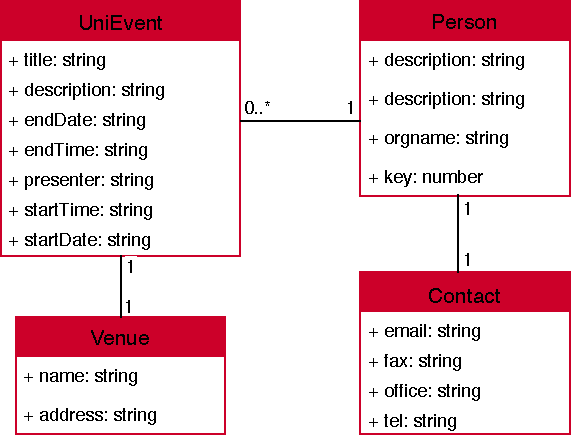
\includegraphics{gfx/Calendar}
\caption{UML-Diagramm der Klassen für die Personensuche und das Veranstaltungsmodul}
\label{fig:Calendar}
\end{figure}
Die Vorgehensweise in diesem Modul unterscheidet sich nur unwesentlich von der in den vorhergehenden Modulen; beim Initialisieren der Komponente wird eine Reihe von Veranstaltungen geladen und weil diese auch in \acs{XML}-Form vorliegen, müssen diese in \acs{JSON}-Objekte übersetzt werden. Neben den bereits im vorhergehenden Kapitel beschrieben Klassen \texttt{Person} und \texttt{Contact} wurden dafür die ebenfalls in Abbildung \ref{fig:Calendar} abgebildeten Klassen \texttt{UniEvent}\footnote{\texttt{/models/uniEvent.ts}} und \texttt{Venue}\footnote{\texttt{/models/venue.ts}}verwendet.

In diesem Modul wurde sich zu Nutze gemacht, dass der \texttt{CalendarService}\footnote{\texttt{/calendar/calendar.service.ts}} global existiert; wurden die Daten geparst, werden sie im Service gespeichert, sodass beim Initialisieren der Komponente zunächst geprüft werden kann, ob die Liste der Veranstaltungen bereits als \acs{JSON}-Array vorliegt. Wie das umgesetzt wurde, zeigt Ausschnitt \ref{calendar} aus dem CalendarComponent\footnote{\texttt{/calendar/calendar-component/calendar.component.ts}}. Nachdem auch hier wieder der Titel der Seite und der Toolbar geändert wurde, wird die Liste der im Service gespeicherten Veranstaltungen abgefragt (\texttt{getEvents()} gibt ein Array vom Typ \texttt{UniEvent} zurück) und geprüft, ob diese leer ist und nur dann die Daten vom Server bezogen(Zeile 4), wobei diese dann natürlich anschließend geparst werden müssen.

\begin{lstlisting}[float, floatplacement=h, style=htmlcssjs, caption={Initialiserung des \texttt{CalendarComponent}}, label={calendar}]
ngOnInit() {
  this.setTitle();
  if ((this.events = this.calendarService.getEvents()).length === 0 ) {
    this.calendarService.getEventsFromServer()
      .subscribe(events => {
        this.events = this.calendarService.parseEventsFromXmlToJson(events);
      });
  }
}
\end{lstlisting}
Das Übersetzten der Daten funktioniert hier im Wesentlichen wie bereits in den vorhergehenden Modulen. Eine Schwierigkeit war an dieser Stelle war, dass in der Anwort vom Server Kontaktperson (\texttt{Person}) und Veranstaltungsort (\texttt{Venue}) nicht in die Veranstaltung (\texttt{UniEvent}) ``eingebettet`` sind - sowie es beispielsweise bei den Kontaktdaten der Personen der Fall ist. Stattdessen sind sie jeweils einzeln gelistet. Dies macht aus Sicht der serverseitigen Verwaltung ja auch durchaus Sinn, schließlich sind ```Veranstaltung``, ``Ort`` und ``Person`` drei unabhängige Entitäten, die auch individuell verwaltet werden.

\begin{lstlisting}[float, floatplacement=h, style=htmlcssjs, caption={Ausschnitt aus CalendarService}, label={CalendarService}]
parseEventsFromXmlToJson(response: string): UniEvent[] {
  /*...*/
  this.parsePersonsFromXmlToJson(personsAsXml);
  for (let index = 0; index < eventsAsXml.length; index++) {
    const eventAsXml = eventsAsXml[index];
    const event = new UniEvent();
    const contactKey = (eventAsXml.getElementsByTagName('contact')[0].firstChild as Element).getAttribute('key');
    event.person = this.persons.get(contactKey);
    /*...*/
    this.events.push(event);
  }
  this.sortEvents(this.events);
  return this.events;
}

private parsePersonsFromXmlToJson(personsAsXml: NodeListOf<Element>) {
  for (let index = 0; index < personsAsXml.length; index++) {
 /*...*/
    this.persons.set(key, person);
  }
}
\end{lstlisting}
Für die weitere Verabeitung wurden der Veranstaltung die zugehörige Ansprechperson und sowie der Veranstaltungsort als ``Kindobjekte`` zugewiesen. Da die \texttt{Event}-Objekte logischerweise die Kontaktperson sowie den Veranstaltungsort über deren ID referenzieren, wurde dies wie in den zwei Funktionen, welche in Ausschnitt \ref{CalendarService} wiedergegeben werden. In der Funktion zum ``Übersetzten`` der Daten werden zunächst die Personen und die Räume (hier nicht gezeigt) verarbeitet, wobei dies jeweils in weiteren, äquivalenten Methoden geschieht. In beiden Fällen wird über die Liste der Elemente iteriert, diese geparst und anschließend in einer Map gespeichert, wobei die Person bzw. der Raum der zugehörigen ID zugewiesen wird (Zeile 20). Da in den Events ebenjene IDs hinterlegt sind (Zeile 8), können über diese dem erzeugten \textit{UniEvent}-Objekt das entsprechende \texttt{Person} - bzw \texttt{Venue}-Objekt zugewiesen werden (Zeile 9). Danach wird das \texttt{UniEvent}-Objekt einer Liste hinzugefügt und diese vor der Rückgabe chronologisch sortiert.

\begin{lstlisting}[float, floatplacement=h, style=htmlcssjs, caption={Ausschnitt des Templates der }, label={Events}]
<mat-accordion>
  <mat-expansion-panel *ngFor="let event of events">
    <mat-expansion-panel-header >
      <mat-panel-title [ngClass]="panelOpenState? 'expanded' : 'collapsed' ">
        <span class="date">{{ event.startDate | date: 'dd.MM' }}</span> {{ event.title }}
      </mat-panel-title>
    </mat-expansion-panel-header>
    <mat-list>
    <!-- ... -->
     <mat-list-item>
        <mat-icon svgIcon="person" color="primary"></mat-icon>
        <a routerLink="/Personensuche/{{ event.person.key }}">
          Kontakt
        </a>
      </mat-list-item> 
    </mat-list>
  </mat-expansion-panel>
</mat-accordion>
\end{lstlisting}
Wie im vorherigen Kapitel angedeutet, wurde für das Layout dieser Komponente ein Akkordeonelement verwendet. Ein Ausschnitt des Templates\footnote{\texttt{/calendar/calendar-component/calendar.component.html}} ist in Beispiel \ref{Events} angegeben. Ein Element, das auf- und zuklappt, wenn man es anklickt, wird eigentlich schon durch den \texttt{mat-expansion-panel}-Tag definiert. Umgibt man dieses mit dem \texttt{mat-accordion}-Tag, so wird zwischen einem aufgeklappten Element und den benachbarten ein \textit{Padding} eingefügt. In einem solchen Panel wird dann ein Kopfbereich mit einem Titel angeben, gefolgt vom Inhalt, der nur im aufgeklappten Zustand sichtbar ist. In diesem Fall handelt es sich um eine Liste der das Event beschreibenden Attribute welche unter anderem auch die Kontaktperson enthält. Im vorhergehenden Kapitel wurde bereits darauf hingewiesen, dass deren Daten hier nicht angezeigt werden. Stattdessen wird ein Link eingefügt, der zur Komponente der Personensuche führt, wobei die ID der Person an den Pfad angehängt wird (Zeile 12). Das Ergebnis sieht dann so aus wie in Abbildung \ref{fig:events}.

\begin{figure}
\begin{subfigure}{.5\textwidth}
  \centering
  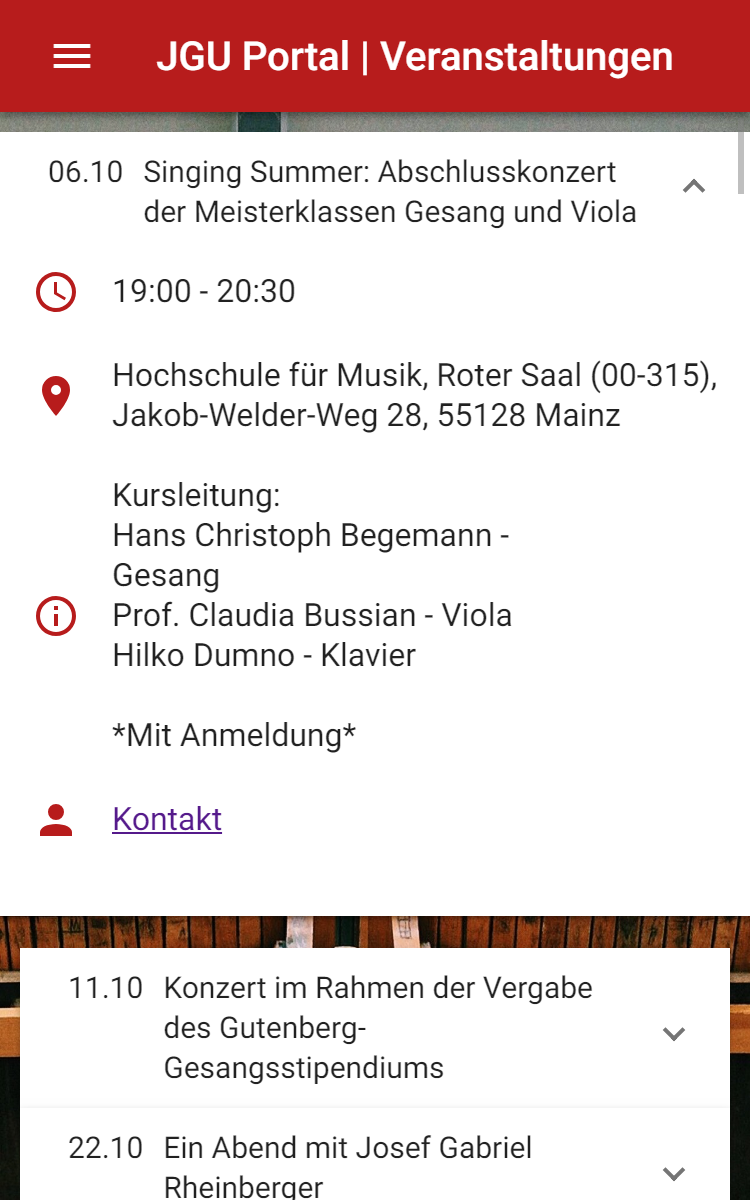
\includegraphics[width=.8\linewidth]{gfx/Events}
  \caption{Ansicht der Veranstaltungen}
  \label{fig:events}
\end{subfigure}%
\begin{subfigure}{.5\textwidth}
  \centering
  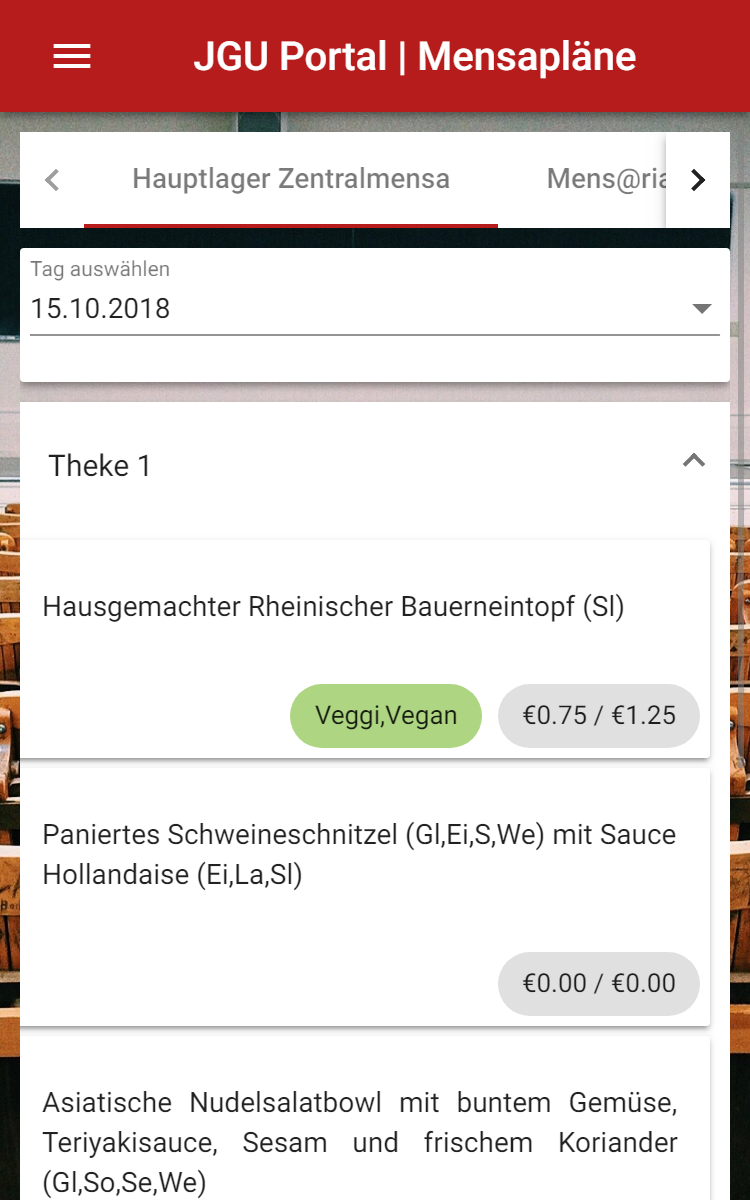
\includegraphics[width=.8\linewidth]{gfx/Mensa}
  \caption{Die Speisepläne der Mensen}
  \label{fig:canteens}
\end{subfigure}
\caption{Das Veranstaltungs- und das Mensamodul}
\label{fig:events+canteens}
\end{figure}
\subsection{Speisepläne}
\label{sec:prog:canteens}
Auch für dieses Modul liegen die Daten im \acs{XML}-Format vor und müssen dementsprechend geparst werden, allerdings sind die Daten hier nicht wirklich modelliert: Empfangen wird eine Liste von Speisen, denen wiederum eine Reihe von Attributen zugeordnet sind - beispielsweise Preis, Inhaltsstoffe oder Ausgabetheke. Zur besseren Verarbeitung sowie Darstellung wurden neben der Klasse \texttt{Meal}\footnote{\texttt{/models/meal.ts}} noch die Klassen \texttt{Canteen}\footnote{\texttt{/models/canteen.ts}} und \texttt{Counter}\footnote{\texttt{/models/counter.ts}} entwickelt - alle dargestellt in Abbildung \ref{MensaUML}. Dabei sind in den empfangenen Daten den Speisen mehr Attribute zugewiesen, als in der \texttt{Meal}-Klasse angegeben: Hier werden nur die Eigenschaften in einen \texttt{Meal}-Objekt gespeichert, die auch tatsächlich angezeigt werden - eine Artikelnummer taucht beispielsweise gar nicht auf.

\begin{figure}[h]
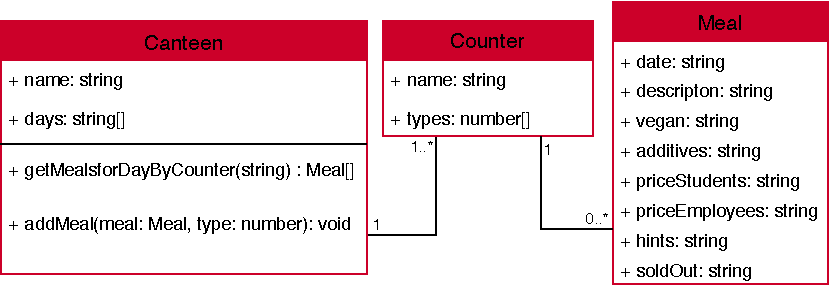
\includegraphics{gfx/MensaUML}
\caption{UML-Diagramm der Klassen für das Mensamoduls}
\label{fig:cannteensUML}
\end{figure}
Beide  Methoden der Klasse \texttt{Canteen} sind in Auszug \ref{Canteen} angegeben. Mit der einen wird ein Gericht der entsprechenden Ausgabe der Kantine zugeordnet und anschließend eine Liste aller Tage, an denen diese Kantine geöffnet ist (also Gerichte erhältlich sind), erstellt. Die andere gibt alle an dem angegeben Tag verfügbaren Speisen - gruppiert nach Ausgabe zurück. Hierfür wird eine Liste für die Rückgabe erstellt, anschließend über die in dieser Mensa enthaltenen Ausgabetheken iteriert und für alle generell dort ausgegebenen Gerichte geprüft, ob sie an dem übergebenen Tag erhältlich sind. Ist das der Fall, wird die jeweilige Speise zu einem neuen \texttt{Counter}-Objekt hinzugefügt. Wurde dies für jede Speise der Theke geprüft, wird diese der Liste für die Rückgabe hinzugefügt. Wurde so für alle Ausgaben verfahren, wird die Liste zurückgegeben.

Weiterhin wurden in einer .json-Datei\footnote{\texttt{/canteen/canteens.json}} alle Mensen auf dem Campus aufgelistet, wobei zu diesen die darin befindlichen Ausgabetheken angegeben sind, welchen wiederum die Typen der an diesen Ausgaben erhältlichen Gerichte zugeordnet sind.

\begin{lstlisting}[float, floatplacement=h, style=htmlcssjs, caption={Auszug aus der Klasse \texttt{Canteen}}, label={Canteen}]
addMeal(meal: Meal) {
  this.counters.forEach(counter => {
    if (counter.types.indexOf(+meal.type) >= 0) {
      counter.meals.push(meal);
    }
  });
  if (this.days.indexOf(meal.date) < 0) {
    this.days.push(meal.date);
  }
}  
getMealsForDayByCounter(day: string): Counter[] {
  const result: Counter[] = [];
  this.counters.forEach(counter => {
    const temp: Counter = new Counter(counter.name);
    counter.meals.forEach(meal => {
      if (meal.date === day) {
        temp.meals.push(meal);
      }
    });
    result.push(temp);
  });
  return result;
}  
\end{lstlisting}

Mit Hilfe dieser drei Klassen können die Daten dann weiterverarbeitet werden, wobei das Parsen im \texttt{CanteenService}\footnote{\texttt{canteen/canteen.service.ts}} auch hier wieder im Grunde so funktioniert, wie in den bisher beschriebenen Fällen. Dazu nur noch ein paar Anmerkungen: Es werden logischerweise nur die Daten derjenigen Speisen weiterverarbeitet, die in einer Mensa auf dem Campus ausgegeben werden. Ebenso werden Daten von Speisen verworfen, die an vergangenen Tagen ausgegeben wurden - dies wird in einer eigenen Methode geprüft. Wurden die Daten eines Gerichts aus den \acs{XML}-Daten ausgelesen, wird dieses - auch wieder in einer eigenen Funktion - in einer \texttt{switch}-Anweisung der entsprechenden Mensa zugeordnet, was über die bereits beschrieben \texttt{addMeal}-Methode der jeweiligen Kantine geschieht.

Die \texttt{ngOnInit}-Methode des \texttt{CanteenComponent}\footnote{\texttt{/canteen/canteen-component/canteen.component.ts}} sieht im Grunde genauso aus, wie die des vorhergehenden Moduls: Auch hier wird zunächst geprüft, ob die Daten bereits im Service als \acs{JSON} vorliegen und nur, falls das nicht der Fall ist, die Daten vom Server bezogen. Außerdem befinden sich in dieser Komponente die zwei in Ausschnitt \ref{CanteenComponent} wiedergegebenen Funktionen. Auch hier wurde ein Registerkartenlayout gewählt, um zwischen den einzelnen Kantinen zu wechseln. Wenn dies geschieht, wird die für dieses Ereignis als \textit{EventListener} definierte Methode \texttt{setActiveCanteen} ausgeführt. In dieser wird zum einen die aktive Mensa neu gesetzt und zum anderen die Liste der Ausgabetheken der neu gewählten Mensa abgefragt, wenn bereits ein Tag aus der Drop-Down-Liste ausgewählt wurde. Das bedeutet, wenn ein Tag ausgewählt wurde und man die Mensa wechselt, werden dort die am gewählten Tag  verfügbaren Gerichte (gruppiert nach zugehöriger Ausgabe) aufgelistet. Ist kein Tag ausgewählt worden, wird dort logischerweise nichts angezeigt.

\begin{lstlisting}[float, floatplacement=h, style=htmlcssjs, caption={Ausschnitt aus \texttt{CanteenComponent}}, label={CanteenComponent}]
setActiveCanteen(event: MatTabChangeEvent) {
  this.selectedCanteen = this.canteens[event.index];
  if (this.selectedDay !== undefined) {
      this.counters  =  this.selectedCanteen.getMealsForDayByCounter(this.selectedDay);
    }
}
handleSelect(event: MatOptionSelectionChange) {
  if (!event.isUserInput) {
    return;
  }
  if (this.selectedCanteen === undefined) {
    this.selectedCanteen = this.canteens[0];
  }
  this.counters = this.selectedCanteen.getMealsForDayByCounter(event.source.value);
}
\end{lstlisting}
Die zweite Methode wird ausgeführt, wenn ein Datum aus aus der Liste ausgewählt wurde. Zunächst wird dort geprüft, ob dieses Event vom Nutzer ausgelöst wurde und anderenfalls verworfen. Da beim erstmaligen Initialisieren noch keine Mensa (aktiv) ausgewählt wurde, wird standardmäßig die erste in der Liste angezeigt und als aktiv gesetzt. Anschließend werden die für den gewählten Tag verfügbaren Gerichte der ``aktiven`` Mensa - gruppiert nach Ausgabetheke - abgefragt.

Im Template\footnote{\texttt{/canteen/canteen-component/canten.component.html}} werden die Theken in den Registerkarten der Kantinen als Akkordeon-Elemente dargestellt, wobei innerhalb dieser Akkordeon-Elemente die ausgegebenen Speisen als Karten aufgelistet sind. Abbildung \ref{fig:canteens} zeigt dieses Layout.

\subsection{Wetter}
\label{sec:prog:weather}
\begin{figure}
\begin{subfigure}{.5\textwidth}
  \centering
  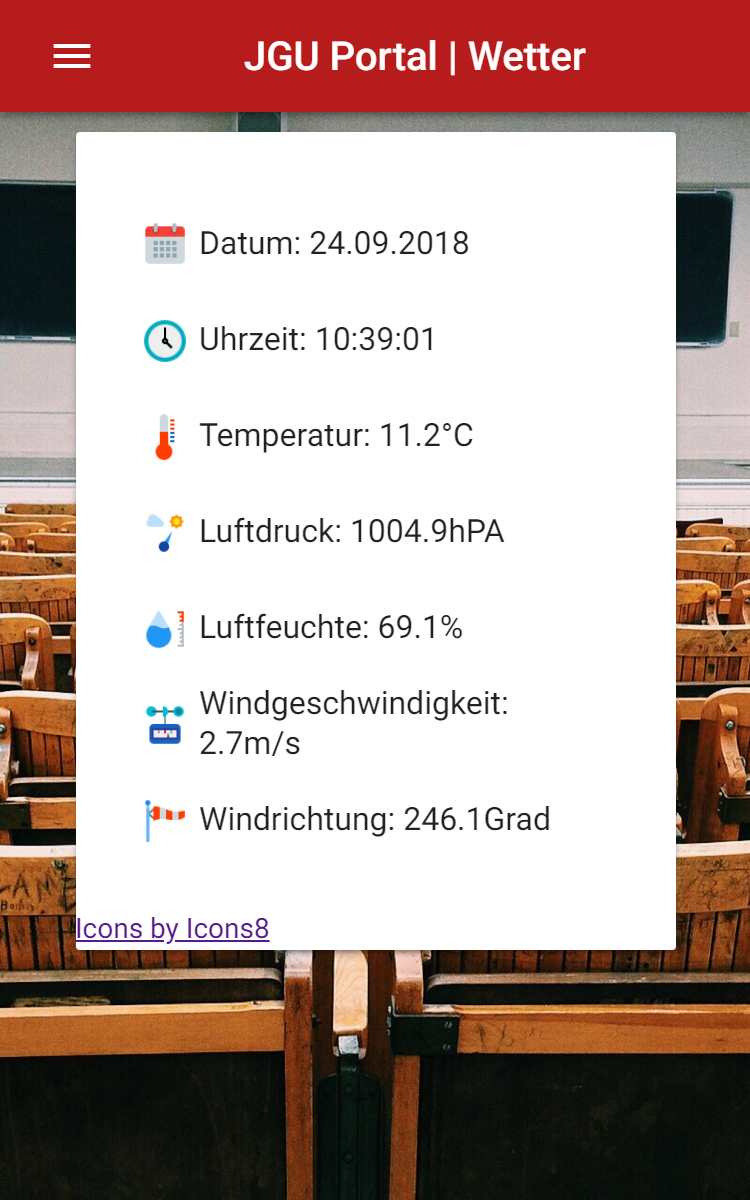
\includegraphics[width=.8\linewidth]{gfx/Wetter}
  \caption{Die Wetterdaten}
  \label{fig:Weather}
\end{subfigure}%
\begin{subfigure}{.5\textwidth}
  \centering
  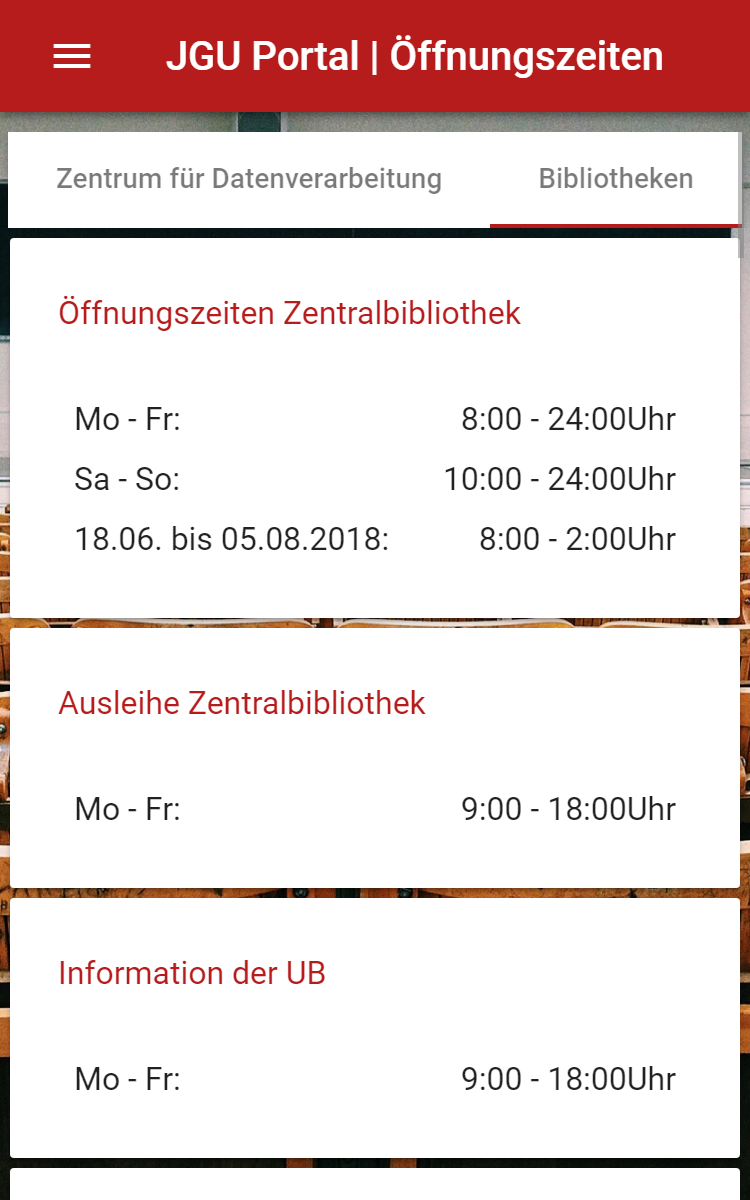
\includegraphics[width=.8\linewidth]{gfx/Zeiten}
  \caption{Öffnungszeiten von ZDV und Bibliotheken}
  \label{fig:Zeiten}
\end{subfigure}
\caption{Wetterdaten und Öffnungszeiten verschiedener Einrichtungen}
\label{fig:}
\end{figure}
Abgesehen davon, dass auch die Wetterdaten im \acs{XML}-Format vorlagen und daher geparst werden mussten, ist dieses Modul recht unkompliziert: Beim Initialisieren der Komponente\footnote{\texttt{/weather/weather-component/weather.component.html}} wird geprüft, ob die Wetterdaten bereits im \texttt{WeatherService}\footnote{\texttt{/weather/weather.service.ts}} gespeichert sind. Ist das der Fall, werden diese genutzt, ansonsten werden sie vom Server bezogen, geparst, im Service gespeichert und dann ins Template eingesetzt. Außerdem werden natürlich auch hier die Titel der Seite und der Toolbar geändert. Abbildung \ref{fig:Weather} zeigt, wie dieses Modul aussieht.

\subsection{Öffnungszeiten}
\label{sec:prog:officeHours}
\begin{figure}[h]
\centering
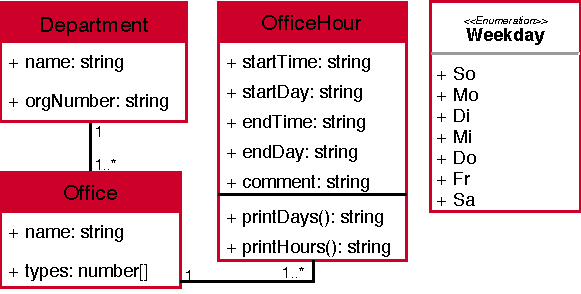
\includegraphics{gfx/Hours}
\caption{UML-Diagramm der Klassen für die Öffnungszeiten}
\label{fig:Hours}
\end{figure}
Da auch in diesem Modul die Daten über das UnivIS bezogen werden, sind sie ebenfalls in \acs{XML}-Form und müssen geparst werden. Für die weitere Verwendung wurden die in Abbildung \ref{fig:Hours} dargestellten Klassen implementiert. Das \textit{Enum} \texttt{Weekday} wird dabei von keiner der anderen Klassen explizit verwendet, sondern dient nur dazu, zu einem Wochentag als Zahl den entsprechenden Wochentag als Kürzel zu erhalten. Ist beispielsweise in der Variablen \texttt{day} als Tag `1` angegeben, kann das Kürzel `Mo` durch \texttt{Weekday[day]} erhalten werden.

Die Liste der \texttt{Department}-Objekte\footnote{\texttt{/models/department.ts}} liegt lokal als \acs{JSON}-Datei vor\footnote{\texttt{/office-hours/Departments.json}}, weil deren IDs benötigt werden, um die Öffnungszeiten (\texttt{officeHour}\footnote{\texttt{/models/officeHour.ts}}) der zugehörigen ``Büros``\footnote{\texttt{/models/office.ts}} abfragen zu können. Momentan sind hier nur Daten für das ZDV sowie für die Bibliotheken hinterlegt, weil für weitere Einrichtungen (noch) keine Daten im UnivIS vorhanden sind. Sollten noch weitere Öffnungszeiten eingepflegt werden, können sie durch Erweitern dieser Datei recht einfach hinzugefügt werden. Beim Parsen der Daten ist hier darauf zu achten, dass neben den regulären Öffnungszeiten auch Ausnahmen angegeben sind - beispielsweise für die vorlesungsfreie Zeit.
Abgesehen davon funktioniert das Übersetzen der Daten auch hier wieder wie zuvor, wobei sich des beschriebenen \textit{Enum} bedient wurde, um aus den Wochentagen als Zahl das entsprechende Kürzel zu erhalten.

Um das Template etwas übersichtlicher zu halten, wurden in der Klasse \texttt{officeHour} die zwei in Ausschnitt \ref{OfficeHours} wiedergegebenen Methoden implementiert. Mit der ersten werden der erste und der letzte Tag, für den diese Öffnungszeit gültig ist, als String formatiert. Ist diese Öffnungszeit nur für einen Tag gültig, wird nur dieser ausgegeben. In der zweiten Methode geschieht analog das gleiche für die entsprechenden Öffnungszeiten. In der Komponente passiert außer dem Abfragen der Daten sowie dem obligatorischen Ändern der Titel weiter nichts.

\begin{lstlisting}[float, floatplacement=h, style=htmlcssjs, caption={Ausschnitt aus der Klasse \texttt{OfficeHour}}, label={OfficeHours}]
  let  res = '';
  if (officeHour.endDay !== undefined) {
    res = officeHour.startDay + ' - ' + officeHour.endDay;
  } else {
    res += officeHour.startDay;
  }
  return res;
}

printHours(officeHour: OfficeHour): string {
  return this.startTime + ' - ' + this.endTime + 'Uhr';
}
\end{lstlisting}
Für das Layout werden auch hier Registerkarten verwendet, die ja bereits vorgestellt wurden. In den Registerkarten sind dann für alle ``Büros`` der jeweiligen Einrichtung Karten aufgelistet, in welchen deren Öffnungszeiten aufgelistet sind. In Abbildung \ref{fig:Zeiten} ist dargestellt wie dieses Modul aussieht.
\subsection{Authentifizierung}
\label{sec:prog:auth}

\begin{lstlisting}[float, floatplacement=h, style=htmlcssjs, caption={Konfiguration für die Authentifizierung}, label={authConfig}]
import { AuthConfig } from 'angular-oauth2-oidc';

export const authConfig: AuthConfig = {
  issuer: 'https://openid.uni-mainz.de',
  redirectUri: window.location.origin + '/signin-oicd',
  clientId: 'jgu.net_portal_website',
  scope: 'openid ',
};
\end{lstlisting}
Die Implementierung der Authentifizierung gestaltet sich dank des Pakets \textit{angular-oauth2-oidc} recht unkompliziert. Nachdem dieses mit \textit{npm} zugewiesen wurde, muss das enthaltene Modul zunächst im \texttt{AppModule} importiert werden (vgl Zeile 13, \ref{appmodule.ts}). Als nächstes muss im Wurzelverzeichnis eine Konfigurationsdatei\footnote{\texttt{auth.config.ts}} erstellt werden. In dieser muss - wie in Ausschnitt \ref{authConfig} wiedergegeben - neben dem \textit{Identity-Provider}, der \texttt{clientId} und dem \texttt{scope} eine \acs{URL} angegeben werden, zu der man nach erfolgreicher Authentifizierung weitergeleitet wird. Zuletzt muss das \texttt{AppComponent} um die in Ausschnitt \ref{auth} angegebene Methode erweitert werden.

In dieser Funktion wird zunächst die eben beschriebene Konfiguration geladen und der Authentifizierungsservice damit initialisiert. Nachdem diesem auch ein neuer \texttt{tokenValidationHandler} initialisiert wurde, wird der eigentliche Authentifizierungsvorgang angestoßen. Wichtig ist noch, dass diese Methode im Konstruktor des \texttt{AppComponent} aufgerufen wird. Diese Konfiguration hat zur Folge, dass man direkt nach Seitenaufruf zum \textit{Identity Provider} weitergeleitet wird. Es ist natürlich auch möglich dies über einen dedizierten Login-Button zu lösen, wobei dafür der Aufruf von \texttt{loadDiscoveryDocumentAndLogin()} aus der eben beschriebenen Methode entfernt und an entsprechender Stelle eingefügt werden muss.

Wie mit diesem Paket Anfragen getätigt werden können, die einer Authentifizierung bedürfen, wird im nächsten Kapitel erklärt.

\begin{lstlisting}[float, floatplacement=h, style=htmlcssjs, caption={Auslösen der Authentifizierung in \texttt{AppComponent}}, label={auth}]
private configureWithNewConfigApi() {
  this.oauthService.configure(authConfig);
  this.oauthService.tokenValidationHandler = new JwksValidationHandler();
  this.oauthService.loadDiscoveryDocumentAndLogin();
}
\end{lstlisting}
\subsection{Bibliotheksausweis}
\label{sec:prog:bibID}
Da für den Bibliotheksausweis eine Authentifizierung notwendig ist, muss bei der Anfrage ein \textit{Header} mitgeschickt werden. Wie dies funktioniert, ist in Ausschnitt \ref{BibAuth} dargestellt. Soll eine ID angefragt werden, wird einer \texttt{Header} erzeugt, in welchen das vom \textit{Identitiy Provider} erhaltene \textit{AccessToken} eingesetzt wird. Der Header kann dann dem \textit{Request} - wie in Zeile 5 dargestellt - mitgegeben werden. Zusätzlich wird angegeben, dass ein Objekt der Klasse \texttt{BibId}\footnote{\texttt{/models/bibId.ts}} erwartet wird.

\begin{lstlisting}[float, floatplacement=h, style=htmlcssjs, caption={Anfrage mit Header am Beispiel des Bibliotheksausweises}, label={BibAuth}]
getLibraryId(): Observable<BibId> {
  const headers = new HttpHeaders({
    'Authorization': 'Bearer ' + this.oauthService.getAccessToken()
  });
  return this.http.get<BibId>(url, { headers: headers});
}
\end{lstlisting}
Hat man auf diese Weise eine ID erhalten, soll mit dieser ein Strichcode erzeugt werden. Mit dem hierfür verwendeten Paket \textit{ngx-barcode} ist das so einfach, wie in Ausschnitt \ref{BibId} dargestellt. Der Komponente \texttt{ngx-barcode} müssen lediglich der darzustellende Wert sowie dessen Format mittels \textit{Attribute Binding} zugewiesen werden. Optional kann angegeben werden, dass der dargestellte Wert ebenfalls unter dem Strichcode  angezeigt werden soll. Ist dieser Wert undefiniert, weil kein Bibliotheksausweis hinterlegt ist, wird ein entsprechender Hinweis angezeigt. Außerdem wird eine Ladeanimation angezeigt, solange es sich \texttt{libraryId} noch um einen leeren String handelt, mit welchem dieses Attribut initialisiert wird. Wurde eine Antwort empfangen, enthält diese Variable entweder die ID, welche dann angezeigt wird, oder sie wird auf \texttt{undefined} gesetzt. In beiden Fällen wird dann zumindest die Grafik angezeigt.

\begin{lstlisting}[float, floatplacement=h, style=htmlcssjs, caption={Template für den Bibliotheksausweis}, label={BibId}]
<mat-card *ngIf="libraryId !== ''; else loading">
  <mat-card-content>
    <img src="/assets/img/LogoUB.jpg" alt="" width="290px">
    <ngx-barcode *ngIf="libraryId !== undefined; else noId"
                 [bc-value]="libraryId" [bc-format]="format" [bc-display-value]="true">
    </ngx-barcode>
    <ng-template #noId>
      <div>Kein Bibliotheksausweis hinterlegt.</div>
    </ng-template>
  </mat-card-content>
</mat-card>
<ng-template #loading><mat-spinner></mat-spinner></ng-template>

\end{lstlisting}
\begin{figure}
\begin{subfigure}{.5\textwidth}
  \centering
  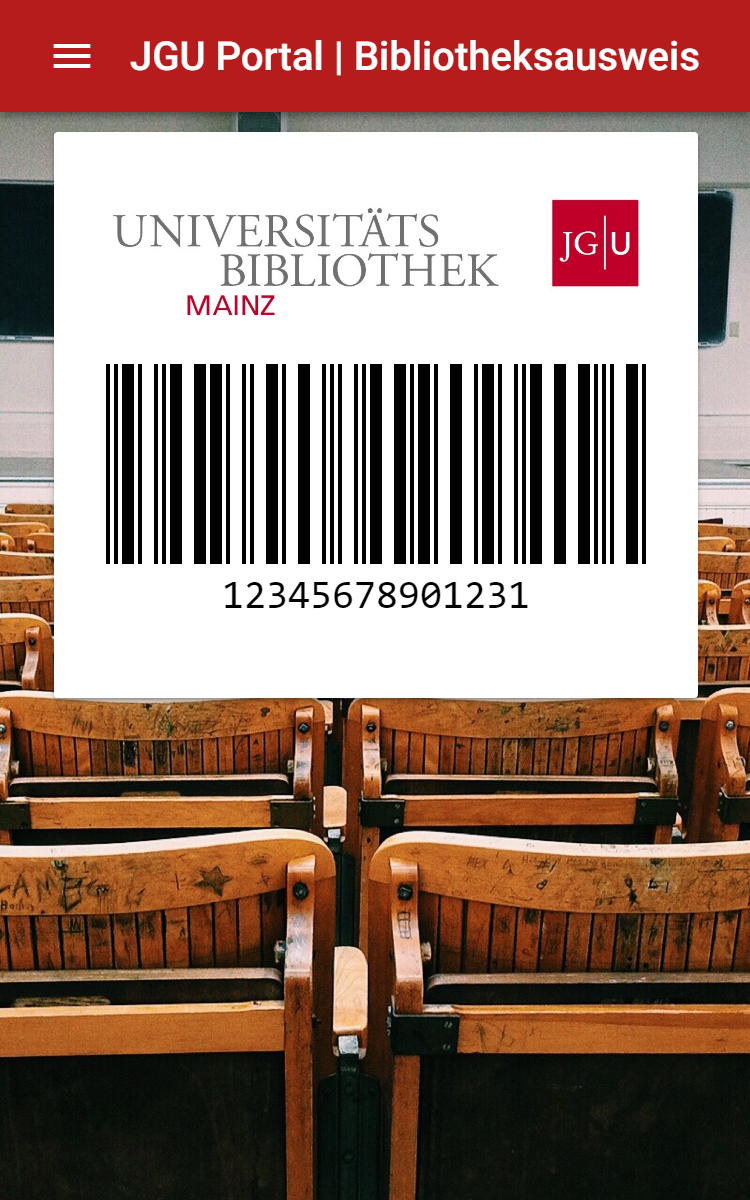
\includegraphics[width=.8\linewidth]{gfx/BibID}
  \caption{Exemplarischer Bibliotheksausweises}
  \label{fig:BibId}
\end{subfigure}%
\begin{subfigure}{.5\textwidth}
  \centering
  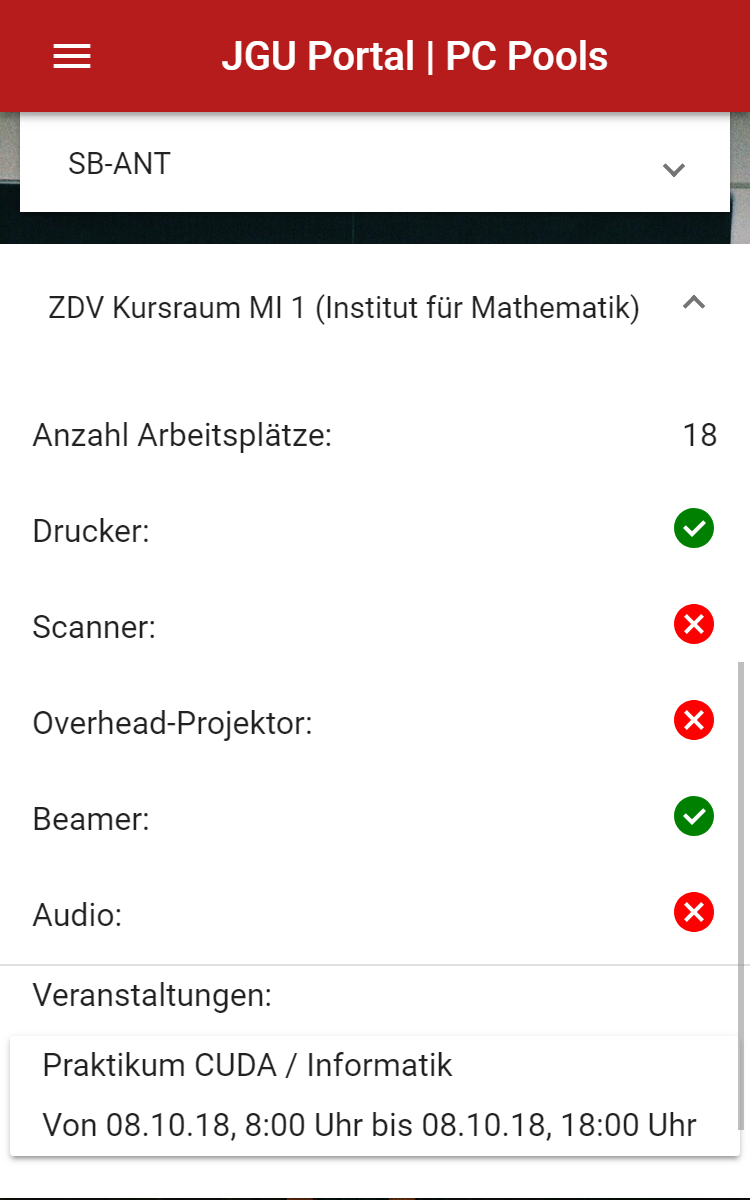
\includegraphics[width=.8\linewidth]{gfx/PC-Pools}
  \caption{Ansicht der PC-Pools}
  \label{fig:Pc-Pools}
\end{subfigure}
\caption{Das Bibliotheksausweis- und das PC-Pool-Modul}
\label{fig:Bib+Pc}
\end{figure}

\subsection{PC-Pools}
\label{sec:prog:pcpools}
\begin{figure}[h]
\centering
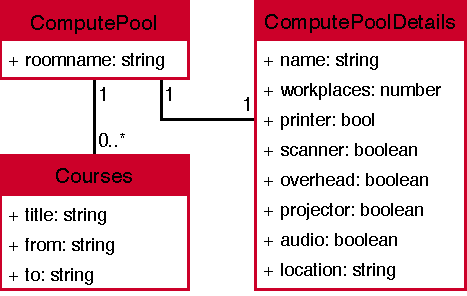
\includegraphics{gfx/ComputePools}
\caption{UML-Diagramm der Klassen für das PC-Pool-Modul}
\label{fig:PoolUml}
\end{figure}
Die Daten für dieses Modul sind zweigeteilt: In einer lokalen \acs{JSON}-Datei\footnote{\texttt{/pc-pools/computePools.json}} sind die PC-Pools mit deren Ausstattung aufgelistet und die Kurse werden über eine API bezogen - ebenfalls als \acs{JSON}. Die Daten sind in den Klassen, welche in Abbildung \ref{fig:PoolUml} abgebildet sind, modelliert. Strenggenommen ist für die Details der Räume keine eigene Klasse notwendig. Für die weitere Verarbeitung ist diese Kapselung jedoch von Vorteil. Warum das so ist lässt sich am Ausschnitt \ref{pcPools} aus dem \texttt{PcPoolsService}\footnote{\texttt{/pc-pools/pc-pools.service.ts}} erläutern.

In diesem ist zunächst die Methode aufgeführt, über welche die Daten von der \acs{API} bezogen werden. Hierbei fällt auf, dass die Daten nicht als Array vom Type \texttt{Course}\footnote{\texttt{/models/course.ts}} empfangen werden. Stattdessen sind sie in Objekte gekapselt, in welchen der Name des zugehörigen PC-Pools hinterlegt ist. Der Einfachheit halber werden diese Objekte ebenfalls als \texttt{ComputePool}\footnote{\texttt{/models/computePool.ts}} bezeichnet - serverseitig gibt es ja keine Typisierung. Dadurch gibt es aber sowohl die lokale gespeicherte Liste der Räume \textit{mit} \texttt{computePoolDetails}\footnote{\texttt{/models/computePoolDetails.ts}} und die von der API erhaltene Raumliste \textit{ohne} Details.

Die ``Verschmelzung`` beider Listen wird ausgeführt, indem vor der Weitergabe der Liste an das \texttt{PcPoolsComponent}\footnote{\texttt{/pc-pools/pc-pools-component/pc-pools.component.ts}} ein \textit{Mapping} in einer \textit{Pipe} stattfindet (Zeile 5). In der durch das Mapping aufgerufenen Methode wird für jedes erhaltene \texttt{ComputePool}-Objekt das lokale gespeicherte Objekt mit demselben Raumnamen gesucht und die Kurse übertragen. Anschließend wird die, um die Veranstaltungen ergänzte, lokale Liste zurückgegeben. Abbildung \ref{fig:Pc-Pools} zeigt, wie die erhaltenen Daten dann angezeigt werden.

\begin{lstlisting}[float, floatplacement=h, style=htmlcssjs, caption={Ausschnitt aus PcPoolsService}, label={pcPools}]
getComputePools(): Observable<ComputePool[]> {
  return this.http.get<ComputePool[]>(proxy + url)
    .pipe(
      map(computePools => this.addDetailsToComputePools(computePools))
    );
}
private addDetailsToComputePools(computePools: ComputePool[]) {
  this.pcPools.forEach(pool => {
    computePools.forEach(computePool => {
      if (pool.roomName === computePool.roomName) {
        pool.events = computePool.events;
      }
    });
  });
  return this.pcPools;
}
\end{lstlisting}

\section{Umwandlung in eine Progessive Web App}
\label{sec:prog:pwa}

Nachdem alle Inhalte eingebaut wurden, bleibt nur noch, die bis hierher entwickelte Web-App in eine \acl{PWA} zu verwandeln. Mit Verwendung des Pakets \textit{@angular/pwa} muss im Grunde lediglich der Befehl \texttt{ng add @angular/pwa} des Angular-\acs{CLI} ausgeführt und dieses Paket somit installiert werden. Hierbei geschehen im Wesentlichen drei Dinge:
\begin{enumerate}
\item Im Wurzelverzeichnis des Projekts wird die Datei \texttt{ngsw-config.json} erstellt.
\item Im Verzeichnis \texttt{/src/} wird die Datei \texttt{manifest.json} erstellt.
\item Im \texttt{AppModule} wird das ServiceWorker-Modul importiert sowie ein entsprechendes Skript registriert (vgl. Ausschnitt \ref{appmodule.ts}, Zeile 14).
\end{enumerate}

Damit erhält man - nach Abschluss des Build-Prozesses mittels \texttt{ng build} - im Grunde schon eine den Spezifikationen entsprechende \textit{\acl{PWA}} - vorausgesetzt, sie wird via HTTPS ausgeliefert. Allerdings sollten die automatisch im Verzeichnis \texttt{/src/assets/icons} erzeugten Icons ersetzt, die Eigenschaften der Web-App in \texttt{manifest.json} angepasst, und in \texttt{ngsw-config.json} die im Cache zu speichernden Ressourcen definiert werden. Im Falle dieses Projekts wurde die Manifest-Datei - wie in Ausschnitt \ref{manifest} dargestellt - angepasst. Dabei werden als Haupt- bzw. Hintergrundfarbe die Rot- und Grau-Töne des JGU-Corporate-Design gewählt und die Icons durch das JGU-Logo ersetzt - die vorgegebenen Pfade bleiben unverändert. Außerdem wurde ein kurzer und ein langer Titel gesetzt, sowie angegeben, dass die Seite als eigenständige Anwendung ausgeführt werden soll, wenn der Nutzer dies wünscht. Die Parameter \texttt{scope} und \texttt{start\_url} bleiben unverändert, weil es sich hier um eine \acl{SPA} handelt, sodass logischerweise alle Unterseiten Teil der Anwendung sind und beim Öffnen der Anwendung immer zum Wurzelpfad navigiert werden soll.

\begin{lstlisting}[float, floatplacement=h, style=htmlcssjs, caption={Ausschnitt aus \texttt{manifest.json}}, label={manifest}]
{
  "name": "Studierendenportal JGU Mainz",
  "short_name": "JGU Portal",
  "theme_color": "#b71c1c",
  "background_color": "#fafafa",
  "display": "standalone",
  "scope": "/",
  "start_url": "/",
  "icons": [
  /* */
  ]
}
\end{lstlisting}
In der Konfigurationsdatei für den Service Worker bleiben die vordefinierten Parameter für statischen \textit{Assets} - also für Bilder, Stylesheets und Skripte sowie für das HTML-Dokument - unverändert. Sollten weitere solcher Datein in einem anderen Ordner hinzugefügt werden, so müssen keine vollständigen Dateipfade angegeben werden. Es reicht, ein Verzeichnis hinzuzufügen sowie mit einem oder zwei Sternchen (`*`) zu definieren, ob nur der Inhalt des Verzeichnisses selbst oder auch alle weiteren Unterverzeichnisse gecachet werden soll(en). Beim Build-Prozess werden dann automatisch für alle so definierten Dateien die Pfade generiert und hinzugefügt.

Zuletzt können noch \texttt{dataGroups}\cite{SW-Config} definiert werden. Dabei wird für eine Liste von \acsp{URL} angegeben, nach welchen Kriterien diese im Cache gespeichert bzw. vom Service Worker verarbeitet werden sollen. In diesem Beispiel wird mit \texttt{maxSize} angeben, dass von den über diese beiden \acsp{URL} bezogenen Ressourcen nur zwei Einträge gespeichert werden sollen, die außerdem höchstens 24 Stunden lang gespeichert werden. Weiterhin wird definiert, dass zunächst versucht werden soll, eine aktuelle Version der Daten von der entsprechenden Quelle zu beziehen. Erst wenn nach 30 Sekunden - dem definierten ``Timeout`` - keine Antwort erhalten wurde soll auf eine im Cache gespeichert Version zurückgegriffen werden. Alternativ kann als Strategie auch ``performance`` gewählt werden, wodurch primär versucht wird, auf gespeicherte Datensätze zurückzugreifen. Auf gleiche Weise wird für alle anderen \acsp{URL} verfahren, wobei natürlich auch anderer Optionen gewählt wurden.
\begin{lstlisting}[float, floatplacement=h, style=htmlcssjs, caption={Exemplarische Konfiguration des Service Worker}, label={ngsw.config}]
"dataGroups": [
  {
    "name": "news",
    "urls": [
      "https://www.uni-mainz.de/32.php",
      "https://www.zdv.uni-mainz.de/feed/",
    ],
    "cacheConfig": {
      "maxSize": 2,
      "maxAge": "24h",
      "strategy": "freshness",
      "timeout": "30s"
    }
  }, /*...*/
]  
\end{lstlisting} % INCLUDE: programming
% !TEX root = ../my-thesis.tex
%
\chapter{Zusammenfassung}
\label{sec:conclusion}
\cleanchapterquote{A program is never less than 90\% complete and never more than 95\% complete}{Terry Baker}{}

Dieses Kapitel fasst abschließend die Inhalte der Arbeit zusammen, gibt eine Übersicht darüber, welche Ziele erreicht wurden und welche nicht und gibt dann Ausblick darüber, welche Verbesserungen und Überarbeitungen möglich, nötig oder empfehlenswert sind.
\section{Rückblick}
\label{sec:conclusion:sec1}

In dieser Arbeit wurde mit dem Angular-Framework eine \acf{SPA} entwickelt, welche dann in eine \acf{PWA} ``umgewandelt`` wurde, sodass diese Web-App auf kompatiblen Geräten bzw. in kompatiblen Browsern (fast) genauso wie eine native Anwendung installiert und genutzt werden kann. Dabei wurde zunächst erläutert, welche Idee hinter \acsp{PWA} steckt und was genau eine solche ausmacht. Anschließend wurden Alternativen zu Angular vorgestellt sowie Gemeinsamkeiten und Unterschiede herausgearbeitet. Basierend darauf wurde dann begründet, warum sich Angular von den vorgestellten Libraries bzw. Frameworks am besten für dieses Projekt geeignet hat und außerdem dieses Framework ausführlich beschrieben. Vor der Beschreibung der eigentlichen Programmierung wurden besondere Hindernisse angeführt, die es bei einem solchen Projekt - nicht nur beim Einsatz von Angular, sondern auch von äquivalenten Alternativen - zu überwinden gilt.

Im Wesentlichen wurden fast alle gewünschten Inhalte, die so auch in der ``Uni Mainz``-App zu finden sind, in die Web-App eingebaut. Es fehlt lediglich die Statusübersicht über die Dienste des ZDV (E-Mail, Remote-Desktop, Druckdienste,...). Außerdem funktioniert das Anzeigen der Kontaktdaten der Ansprechperson einer Veranstaltung nicht, wie gewollt. Geplant war, dass einer jeden Veranstaltung ein Link zugeordnet wird, über den man zum Personensuche-Modul gelangt, in welchem dann die entsprechenden Informationen der Kontaktperson angezeigt werden sollen. Da für die Abfrage der Daten einer Person über ihre ID aber ein \textit{key} benötigt wird, der sich in regelmäßigen Abständen ändert, ist dieser Ansatz so nicht praktikabel. Eine Lösung könnte darin bestehen, die bei der Auflistung der Veranstaltungen erhaltenen Informationen über die Kontaktperson an das Personensuche-Modul weiterzuleiten, statt über die ID eine erneute Suche anzustoßen.

Ansonsten sind es Details, die an der ein- oder anderen Stelle ergänzt werden könnten. So wäre es beispielsweise möglich, im Mensamodul Inhaltsstoffe und Allergene der Speisen anzuführen.

Das Umwandeln der Web-App in eine \textit{\acl{PWA}} hingegen - was ja eine Hauptanforderung an dieses Projekt darstellte - war durch das Paket \textit{@angular/pwa} einfach und unkompliziert. Die größte Schwierigkeit bestand hauptsächlich darin, die in \acs{XML}-Form vorliegenden Daten in \acs{JSON}-Form zu ``übersetzen``.

\section{Ausblick}
\label{sec:conclusion:future}
Zu den Inhalten und Funktionen, die noch umgesetzt werden könnten, gehört beispielsweise, dass die Bus- und Straßenbahnhaltestellen nicht auf der Karte markiert werden. Hierauf wurde zunächst verzichtet, weil in dem verwendeten Kartenmaterial bereits Haltestellen eingezeichnet sind. Dennoch wäre es möglich, bei jeder Haltestelle im Busfahrplan-Modul einen Link zu hinterlegen, der zum Kartenmodul weiterleitet, wo dann die Haltestelle auf der Karte markiert würde. Das Busfahrplan-Modul könnte außerdem dahingehend erweitert werden, dass es möglich ist, zu einer Bus- oder Straßenbahnlinie auch den Fahrtverlauf abzufragen.

Weiterhin wäre es denkbar, die Meldungen im Nachrichten-Modul nach Kategorien zu sortieren bzw. dem Nutzer eine Möglichkeit zu bieten, selbst zu entscheiden, welche Kategorien angezeigt werden sollen.

Ebenfalls könnte beispielsweise im Bibliotheksausweis-Modul ein dedizierter Login-Button platziert werden, damit man nicht direkt bei Seitenaufruf weitergeleitet wird. Auf die aktuell umgesetzte Weise ist die Web-App offline quasi nicht möglich, da ohne Internetverbindung logischerweise auch keine externe Authentifizierung möglich ist.

Ein weiterer verbesserungsfähiger Punkt ist das Design bzw. das Layout mancher Module. Es wurde zwar stets versucht, ein für alle Bildschirmgrößen praktikables Layout zu finden, auf Grund der unterschiedlich gearteten Daten war dies aber teilweise nicht ganz einfach. Bei den Veranstaltungen beispielsweise kann die Beschreibung einen einzigen Satz umfassen - aber auch einen ganzen Absatz. Hier ein Layout zu finden, dass beiden Szenarien gerecht wird und nicht in dem einen Fall zu viel und im anderen zu wenig Platz beansprucht - und zwar auf großen, wie auf kleinen Displays - ist mitunter nicht ganz einfach. Das liegt aber genauso wenig an Angular selbst, wie es bei den nicht ganz optimal organisierten Stylesheets der Fall ist.

Obwohl Angular ``testgetriebenes Programmieren`` unterstützt bzw. ermöglicht, wurde hierauf  zugegebenermaßen verzichtet; es könnten dementsprechend noch ein paar Testfälle implementiert werden um sicherzustellen, dass alle Randfälle bedacht wurden. Genauso wäre an ein paar Stellen besseres ``Error-Handling`` - also das Behandeln von \textit{Exceptions} - empfehlenswert. Zwar wurde vor allem beim Parsen der \acs{XML}-Daten darauf geachtet, (möglichst) alle Spezialfälle abzudecken, es ist aber durchaus möglich, dass hier Fehler durch nicht bedachte Szenarien entstehen.





 % INCLUDE: conclusion
\cleardoublepage

% --------------------------
% Back matter
% --------------------------
{%
\setstretch{1.1}
\renewcommand{\bibfont}{\normalfont\small}
\setlength{\biblabelsep}{0pt}
\setlength{\bibitemsep}{0.5\baselineskip plus 0.5\baselineskip}
\printbibliography[nottype=online]
\printbibliography[heading=subbibliography,title={Webseiten},type=online,prefixnumbers={@}]
}
\cleardoublepage

\listoffigures
\cleardoublepage

\listoftables
\cleardoublepage

% !TEX root = ../my-thesis.tex
%
\pagestyle{empty}
\hfill
\vfill
\pdfbookmark[0]{Colophon}{Colophon}
\section*{Colophon}

This thesis was typeset with \LaTeXe.
It uses the \textit{Clean Thesis} style developed by Ricardo Langner.
The design of the \textit{Clean Thesis} style is inspired by user guide documents from Apple Inc.

Download the \textit{Clean Thesis} style at \url{http://cleanthesis.der-ric.de/}.

\cleardoublepage

% !TEX root = ../my-thesis.tex
%
%************************************************
% Declaration
%************************************************
\pdfbookmark[0]{Declaration}{Declaration}
\chapter*{Declaration}
\label{sec:declaration}
\thispagestyle{empty}

I hereby declare that I have written the present thesis independently and without use of other than the indicated means. I also declare that to the best of my knowledge all passages taken from published and unpublished sources have been referenced. The paper has not been submitted for evaluation to any other examining authority nor has it been published in any form whatsoever.

\bigskip

\noindent\textit{\thesisUniversityCity, \thesisDate}

\smallskip

\begin{flushright}
	\begin{minipage}{5cm}
		\rule{\textwidth}{1pt}
		\centering\thesisName
	\end{minipage}
\end{flushright}

%*****************************************
%*****************************************

\clearpage
\newpage
\mbox{}

% **************************************************
% End of Document CONTENT
% **************************************************
\end{document}
